\documentclass[
size=17pt,
paper=smartboard,
mode=present,
display=slidesnotes,
style=paintings,
nopagebreaks,
blackslide,
fleqn]{powerdot}

% styles: sailor, paintings
% wj capsules prettybox
% mode = handout or present


\newcommand{\palette}{Moitessier}
% palettes:
%    - sailor: Sea, River, Wine, Chocolate, Cocktail 
%    - paintings: Syndics, Skater, GoldenGate, Moitessier, PearlEarring, Lamentation, HolyWood, Europa, MayThird, Charon 

\newcommand{\cursopequeno}{EC01045 PDS}
\newcommand{\cursogrande}{\Large EC01045 -- Processamento digital de sinais}

\usepackage{amsmath,graphicx,color,amsfonts}
\usepackage[brazilian]{babel}
\usepackage[utf8]{inputenc}
\usepackage{bbding}

\author{Ronaldo de Freitas Zampolo\\FCT-ITEC-UFPA}
\date{ERE 2020}


\pdsetup{
   lf = {\cursopequeno},
   rf = {Análise de sistemas lineares no domínio transformado},
   palette = \palette,randomdots={false},
   cf={\theslide}
}

\title{\cursogrande\\ \vspace{1cm}Análise de sistemas lineares no domínio transformado}


\begin{document}
\maketitle[randomdots={false}]
   \begin{slide}{Agenda}
      \tableofcontents[content=sections]
   \end{slide}

\section{Introdução}
\begin{slide}{Sistema LI e sua caracterização}
\begin{itemize}
   \item Resposta ao impulso
	   \begin{align*}
		   y[n] &= \sum_{k=-\infty}^{\infty}x[k] h[n-k]\\
		        &= h[n]\ast x[n]
	   \end{align*}
   \item Resposta em frequência
	   \begin{equation*}
		   Y(e^{j\omega}) = H(e^{j\omega})X(e^{j\omega})
	   \end{equation*}
   \item Função de transferência
	   \begin{equation*}
		   Y(z) = H(z)X(z)
	   \end{equation*}
\end{itemize}
\end{slide}

\section{Resposta em frequência de sistemas LI}
\begin{slide}{Fase da resposta em frequência e atraso de grupo}
\begin{itemize}
	\item A resposta em frequência $H(e^{j\omega})$ pode ser vista como o ganho (complexo) que o sistema impõe a entradas exponenciais complexas do tipo $e^{j\omega}$
	\item Relação entre entrada e saída no domínio da frequência (Transformada de Fourier)
	   \begin{equation*}
		   Y(e^{j\omega}) = H(e^{j\omega})X(e^{j\omega})
	   \end{equation*}
        \item Magnitude e fase
	   \begin{align*}
		   |Y(e^{j\omega})| &= |H(e^{j\omega})| |X(e^{j\omega})|\\
		   \angle Y(e^{j\omega}) &= \angle H(e^{j\omega}) + \angle X(e^{j\omega})\\
	   \end{align*}
\end{itemize}
\end{slide}

\begin{slide}{Efeitos do atraso de grupo e atenuação}
\begin{itemize}
	\item r
\end{itemize}
\end{slide}

\section{Sistemas caracterizados por equações de diferenças com coeficientes constantes}
\begin{slide}{Representação de sistemas}
   \begin{figure} % exemplo de sistemas de segunda ordem
      \centering
      %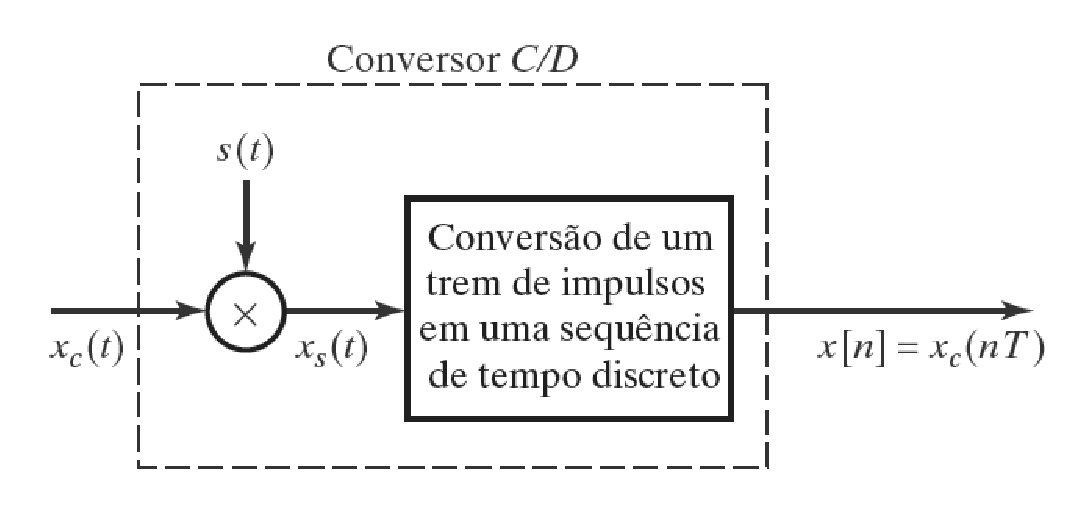
\includegraphics[width=0.7\textwidth]{figs/cd_implem.eps}
   \end{figure}
\end{slide}

\begin{slide}{Estabilidade e Causalidade}
\begin{itemize}
   \item
   \begin{align}
      s(t) &= \sum_{n=-\infty}^{\infty}\delta(t-nT)\\
      x_s(t) &= x_c(t)s(t) \\ &= \sum_{n=-\infty}^{\infty}x_c(nT)\delta(t-nT)
   \end{align}
\end{itemize}
\end{slide}

\begin{slide}{Sistemas inversos}
%\begin{itemize}
%   \item Representa\c c\~ao:
   \begin{figure}
      \centering
      %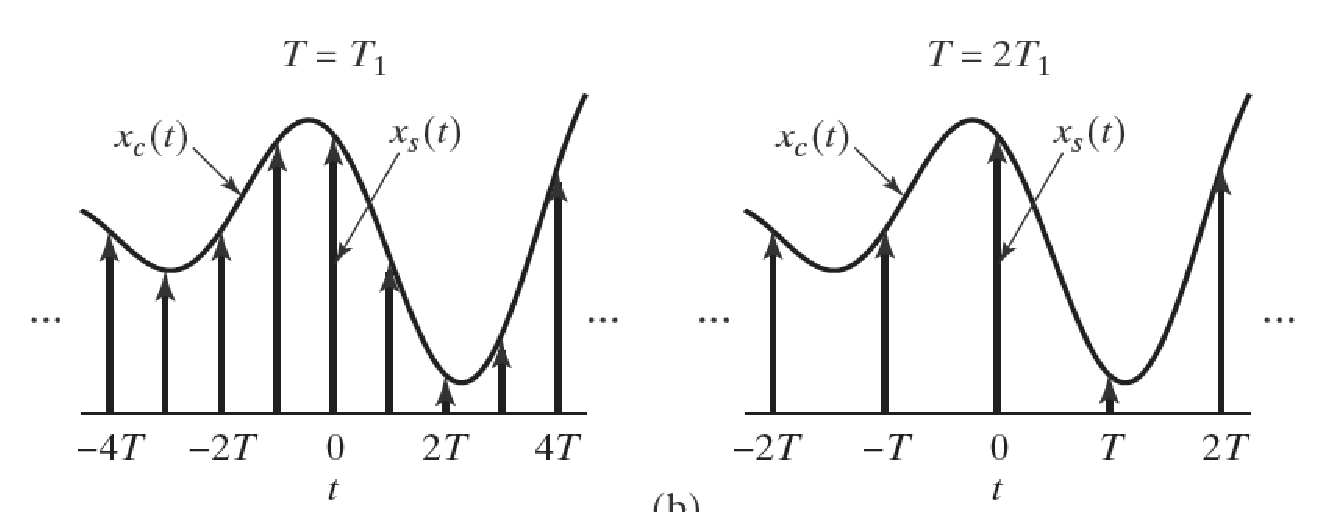
\includegraphics[width=0.7\textwidth]{figs/representacao1.eps}
      %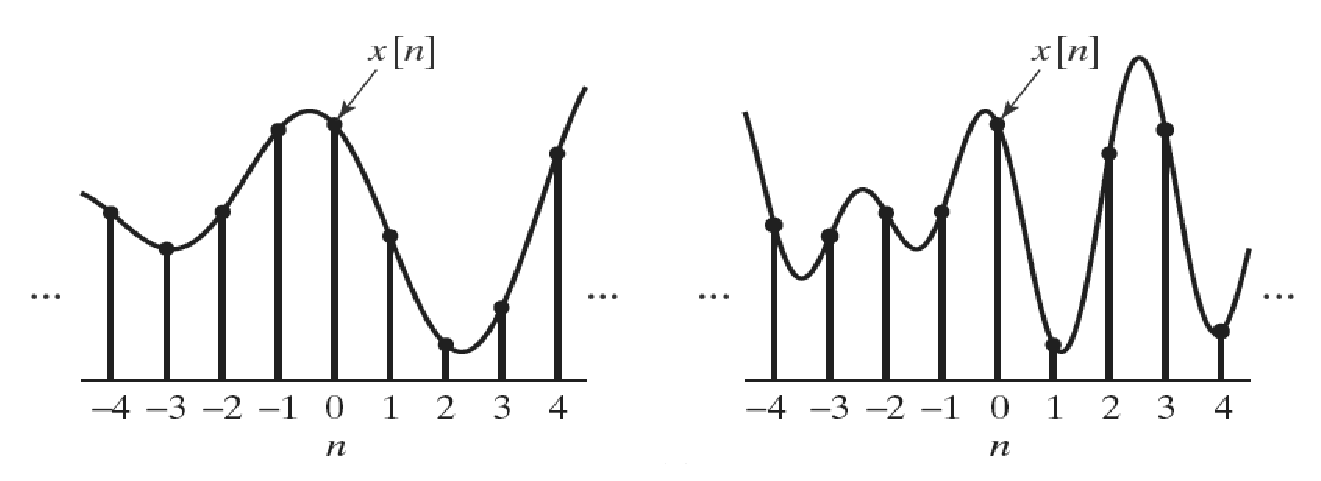
\includegraphics[width=0.7\textwidth]{figs/representacao2.eps}
   \end{figure}
%\end{itemize}
\end{slide}

\begin{slide}{Resposta ao impulso para funções de sistema racionais}
\begin{itemize}
   \item Trem de impulsos:
   \begin{equation}
      s(t) = \sum_{n=-\infty}^{\infty}\delta(t-nT)
   \end{equation}
   \item Sinal cont\'inuo moldulado
   \begin{align}
      x_s(t) &= x_c(t)s(t)\\
             &= \sum_{n=-\infty}^{\infty}x_c(nT)\delta(t-nT)
   \end{align}
\end{itemize}
\end{slide}

\section{Resposta em frequência para funções de sistema racionais}
\begin{slide}{Resposta de sistemas de primeira ordem}
\begin{itemize}
   \item Sinal
   \begin{figure}
      \centering
      %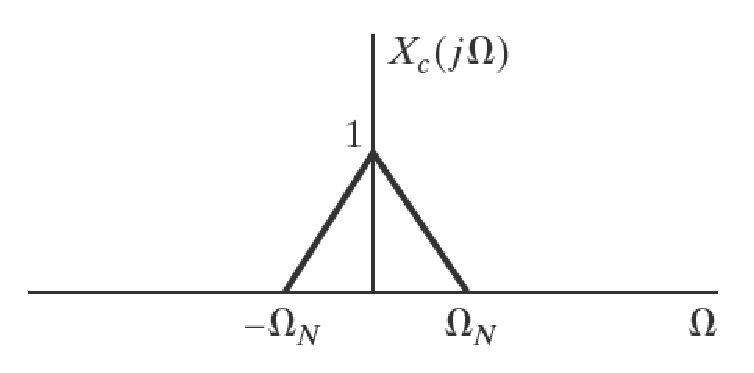
\includegraphics[width=0.7\textwidth]{figs/espectro01a.eps}
      %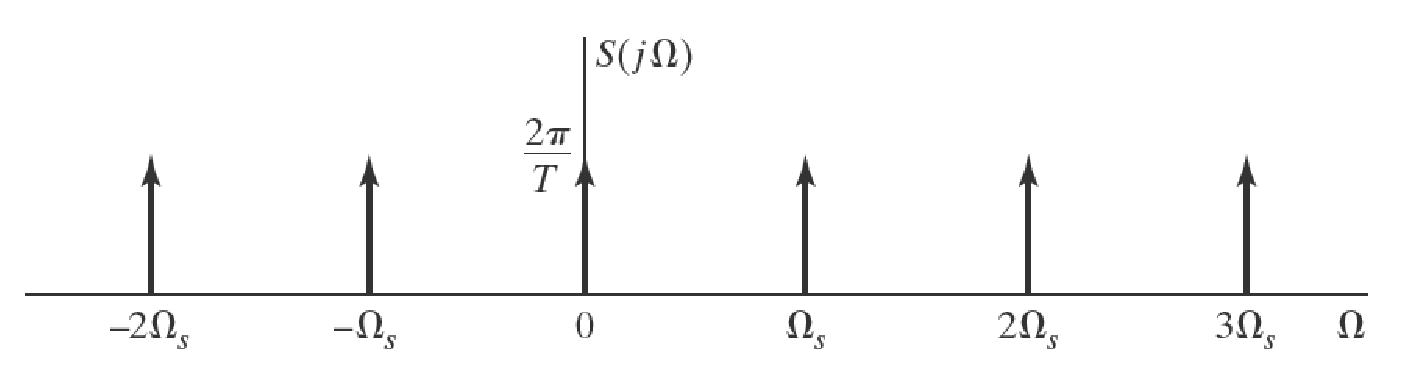
\includegraphics[width=0.7\textwidth]{figs/espectro01b.eps}
   \end{figure}
\end{itemize}
\end{slide}

\begin{slide}{Exemplos com múltiplos polos e zeros}
\begin{itemize}
   \item $\Omega_s-\Omega_N>\Omega_N$
   \begin{figure}
      \centering
      %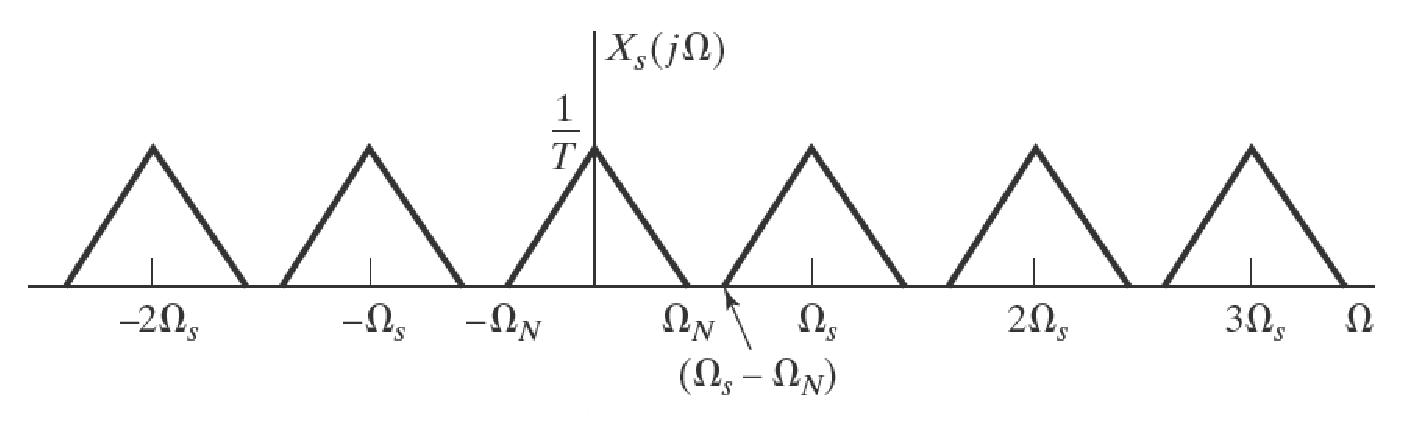
\includegraphics[width=0.9\textwidth]{figs/situacao01.eps}
   \end{figure}
\end{itemize}
\end{slide}

\section{Relação entre magnitude e fase}
\begin{slide}{Estudo da situação 02}
\begin{itemize}
   \item $\Omega_s-\Omega_N<\Omega_N$
   \begin{figure}
      \centering
      %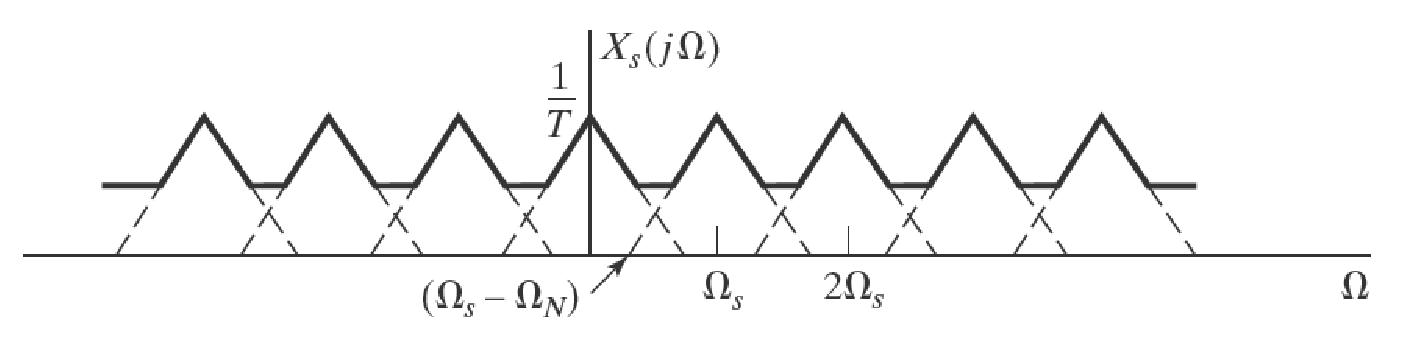
\includegraphics[width=0.9\textwidth]{figs/situacao02.eps}
   \end{figure}
\end{itemize}
\end{slide}

\section{Sistemas passa-tudo}
\begin{slide}{Reconstrução }
\begin{itemize}
   \item Usando %filtro passa-baixas ideal
   \begin{figure}
      \centering
      %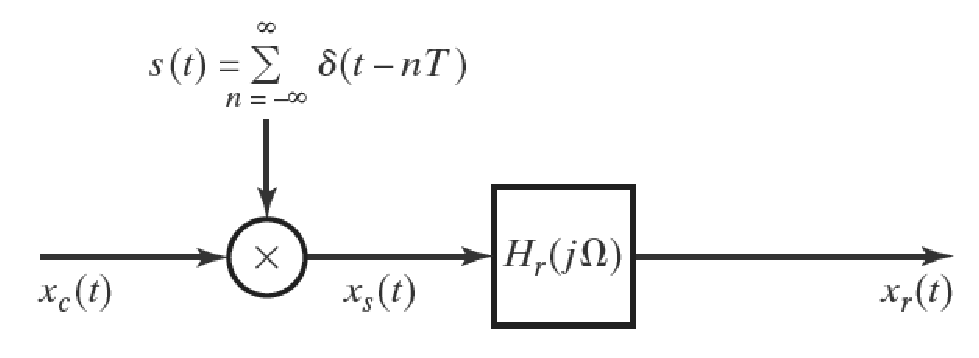
\includegraphics[width=0.7\textwidth]{figs/sistamostragem1.eps}
      %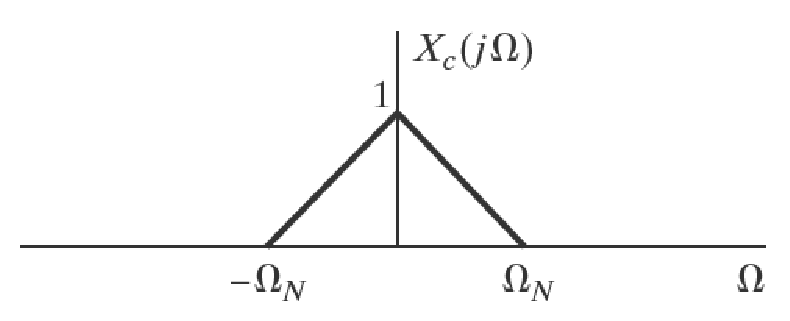
\includegraphics[width=0.7\textwidth]{figs/sistamostragem2.eps}
   \end{figure}
\end{itemize}
\end{slide}

\section{Sistemas de fase mínima}
\begin{slide}{Reconstrução por filtragem 02}
\begin{itemize}
   \item Continuação
   \begin{figure}
      \centering
      %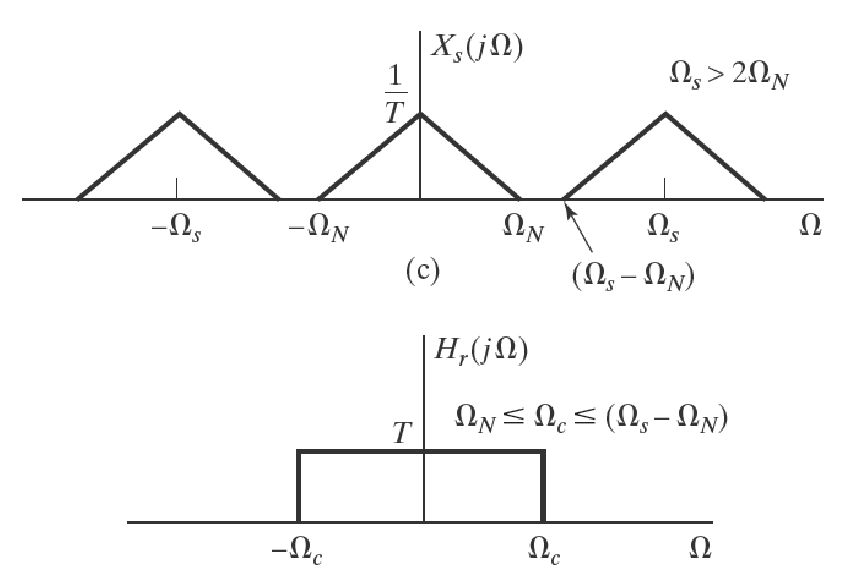
\includegraphics[width=0.7\textwidth]{figs/reconstr01a.eps}
      %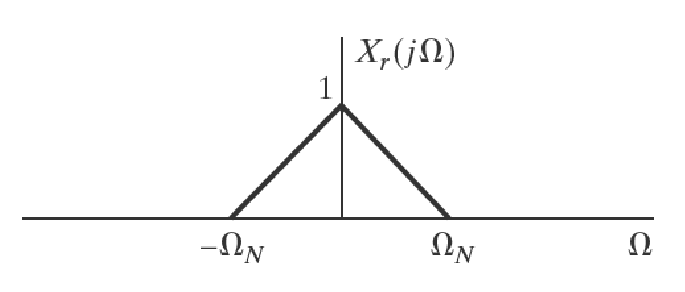
\includegraphics[width=0.9\textwidth]{figs/reconstr01b.eps}
   \end{figure}
\end{itemize}
\end{slide}

\section{Sistemas lineares com fase linear generalizada}
\begin{slide}{uist}
\begin{itemize}
   \item Seja $x_c(t)$ um sinal limitado em frequ\^encia, ou seja
   \begin{equation}
       X_c(j\Omega) = 0, \qquad |\Omega|\geq\Omega_N.
   \end{equation}
   Nesse caso, $x_c(t)$ \'e unicamente determinado por suas amostras $x[n]=x_c(nT)$, desde que 
   \begin{equation}
       \Omega_s = \frac{2\pi}{T}\geq 2\Omega_N.
   \end{equation}
   \item $\Omega_N$: frequ\^encia de Nyquist
   \item $2\Omega_N$: taxa de Nyquist
\end{itemize}
\end{slide}

\begin{slide}{Contínuo $\times$ Discreto}
\begin{itemize}
   \item Rela\c c\~ao entre Transformadas de Fourier 
   \begin{align}
      X_s(j\Omega)   &= \sum_{n=-\infty}^{\infty}x_c(nT)e^{-j\Omega Tn}\\
      X(e^{j\omega}) &= \sum_{n=-\infty}^{\infty}x[n]e^{-j\omega n}\\
      X_s(j\Omega)   &= X(e^{j\omega})|_{\omega=\Omega T}\\
                     &= X(e^{j\Omega T}) \\
                     &= \frac{1}{T}\sum_{k=-\infty}^{\infty}X_c(j(\Omega-k\Omega_s))\\
     X(e^{j\omega})& = \frac{1}{T}\sum_{k=-\infty}^{\infty}X_c\left(j\left(\frac{\omega}{T}-\frac{2k\pi}{T}\right )\right )
   \end{align}
\end{itemize}
\end{slide}

% \begin{slide}{Representa\c c\~ao espectral}
% \begin{itemize}
%    \item Rela\c c\~ao entre Transf. de Fourier (cont.) 
%    \begin{align}
% %       X_s(j\Omega)   &= \sum_{n=-\infty}^{\infty}x_c(nT)e^{-j\Omega Tn}\\
% %       X(e^{j\omega}) &= \sum_{n=-\infty}^{\infty}x[n]e^{-j\omega n}\\
% %       X_s(j\Omega)   &= X(e^{j\omega})|_{\omega=\Omega T}\\
% %                      &= X(e^{j\Omega T}) = \frac{1}{T}\sum_{k=-\infty}^{\infty}X_c(j(\Omega-k\Omega_s))\\
%      X(e^{j\omega})& = \frac{1}{T}\sum_{k=-\infty}^{\infty}X_c\left(j\left(\frac{\omega}{T}-\frac{2k\pi}{T}\right )\right )
%    \end{align}
% \end{itemize}
% \end{slide}


\section{Reconstrução de sinais}
\begin{slide}{Reconstrução ideal}
\begin{itemize}
   \item Diagrama de blocos
   \begin{figure}
      \centering
      %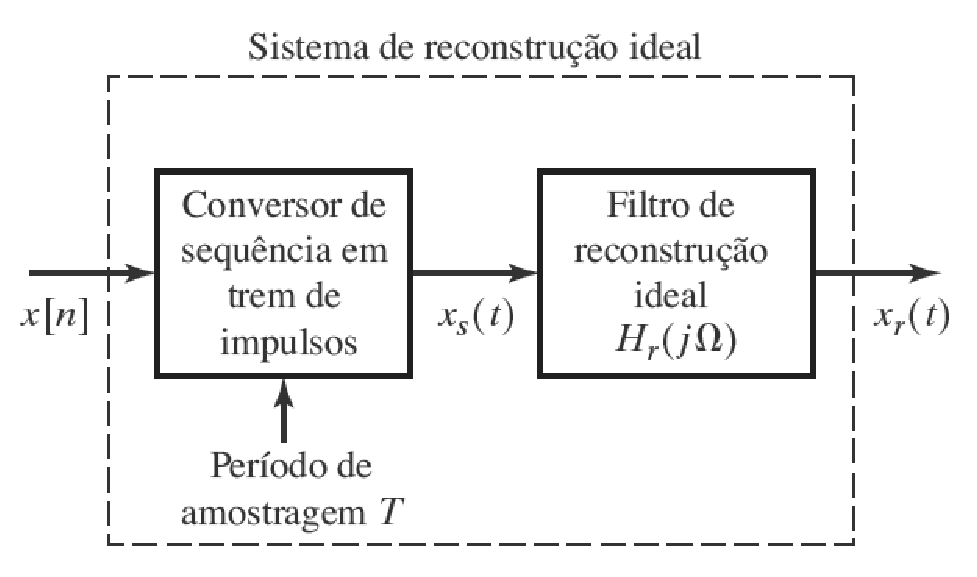
\includegraphics[width=0.7\textwidth]{figs/reconstrblock.eps}
   \end{figure}
\end{itemize}
\end{slide}

\begin{slide}{Filtro de reconstru\c c\~ao ideal}
\begin{itemize}
   \item Representação da resposta em frequência
   \begin{figure}
      \centering
      %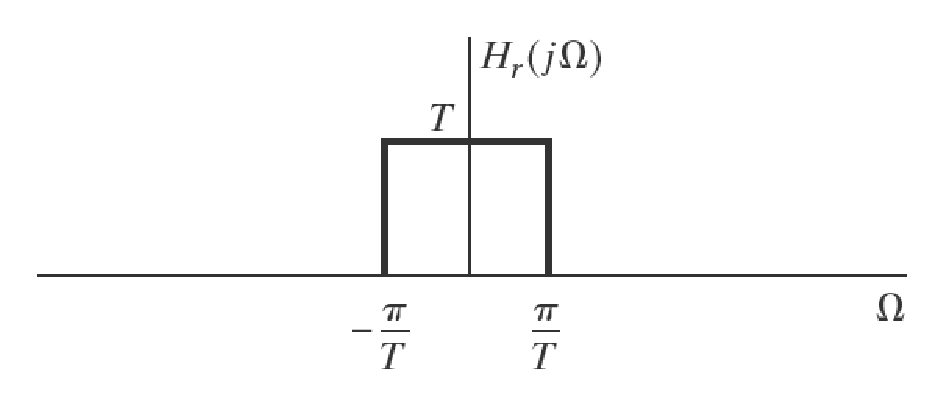
\includegraphics[width=0.9\textwidth]{figs/filtroreconstr.eps}
   \end{figure}
\end{itemize}
\end{slide}

\begin{slide}{Filtro de reconstru\c c\~ao ideal}
\begin{itemize}
   \item Resposta ao impulso
   \begin{figure}
      \centering
      %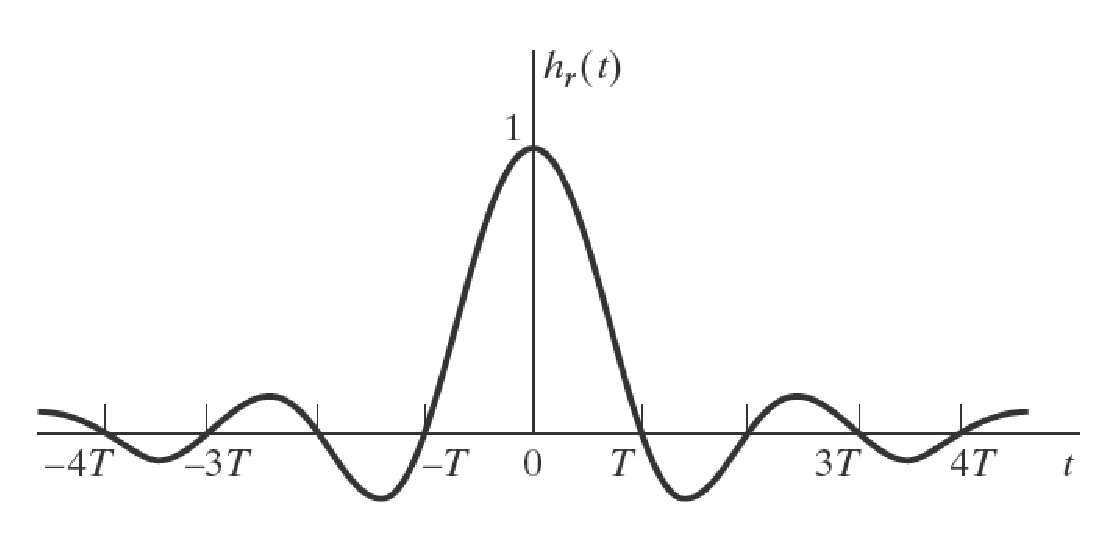
\includegraphics[width=0.9\textwidth]{figs/filtroreconstr01.eps}
   \end{figure}
\end{itemize}
\end{slide}

\begin{slide}{Sinal reconstru\'ido}
\begin{itemize}
   \item Expressões matemáticas
   \begin{align}
      h_r(t) &= \frac{\sin(\pi t/T)}{\pi t/T}\\
      x_r(t) &= x_s(t)*h_r(t)\\
             &= \sum_{n=-\infty}^{\infty}x[n]h_r(t-nT)\\
             &= \sum_{n=-\infty}^{\infty}x[n]\frac{\sin[\pi (t-nT)/T]}{\pi (t-nT)/T}
   \end{align}
\end{itemize}
\end{slide}

\begin{slide}{Reconstru\c c\~ao de sinais}
\begin{itemize}
   \item Sinal cont\'inuo e sinal amostrado
   \begin{figure}
      \centering
      %\includegraphics[width=0.9\textwidth]{figs/reconstr02a.eps}
      %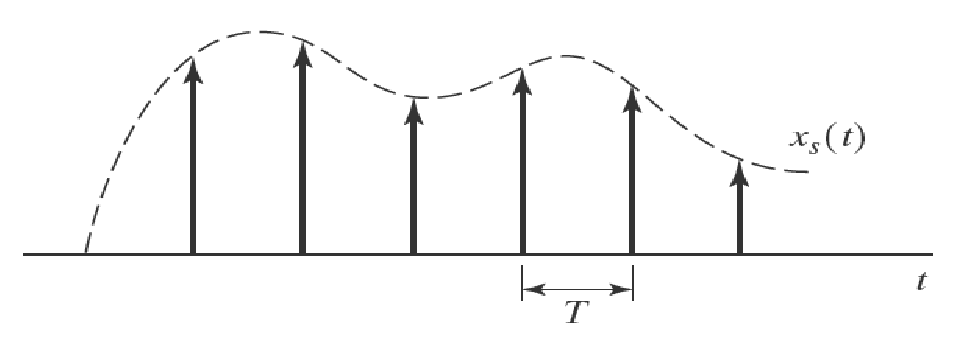
\includegraphics[width=0.9\textwidth]{figs/reconstr02b.eps}
   \end{figure}
\end{itemize}
\end{slide}

\begin{slide}{Reconstru\c c\~ao de sinais}
\begin{itemize}
   \item Sinal reconstru\'ido
   \begin{figure}
      \centering
      %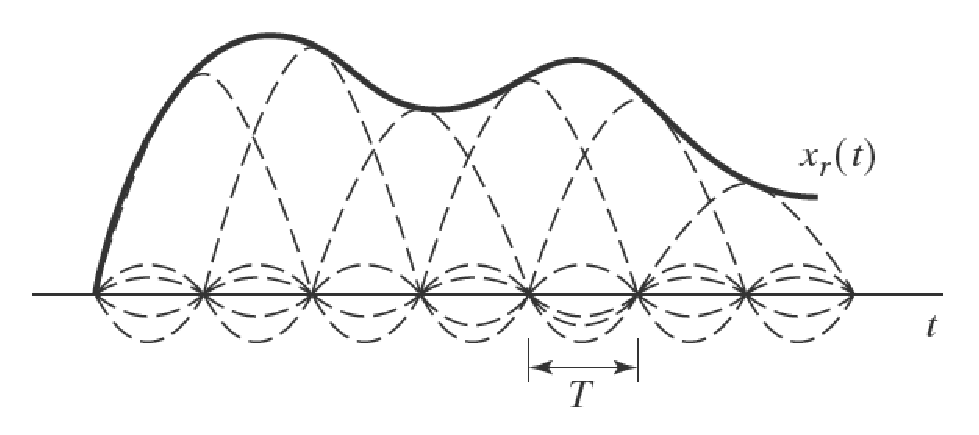
\includegraphics[width=0.9\textwidth]{figs/reconstr03.eps}
   \end{figure}
\end{itemize}
\end{slide}

\begin{slide}{Reconstru\c c\~ao de sinais}
\begin{itemize}
   \item Sinal reconstru\'ido no dom\'inio da frequ\^encia 
   \begin{align}
      X_r(j\Omega) &= H_r(j\Omega)X_s(j\Omega)\\
                   &= \sum_{n=-\infty}^{\infty}x[n]H_r(j\Omega)e^{-j\Omega Tn}\\
                   &= H_r(j\Omega)X(e^{j\Omega T})             
   \end{align}
\end{itemize}
\end{slide}


\section{Processamento discreto de sinais contínuos}
\begin{slide}{Proc. discreto de sinais cont\'inuos}
\begin{itemize}
   \item Diagrama de sistema de processamento discreto de sinais cont\'inuos
   \begin{figure}
      \centering
      %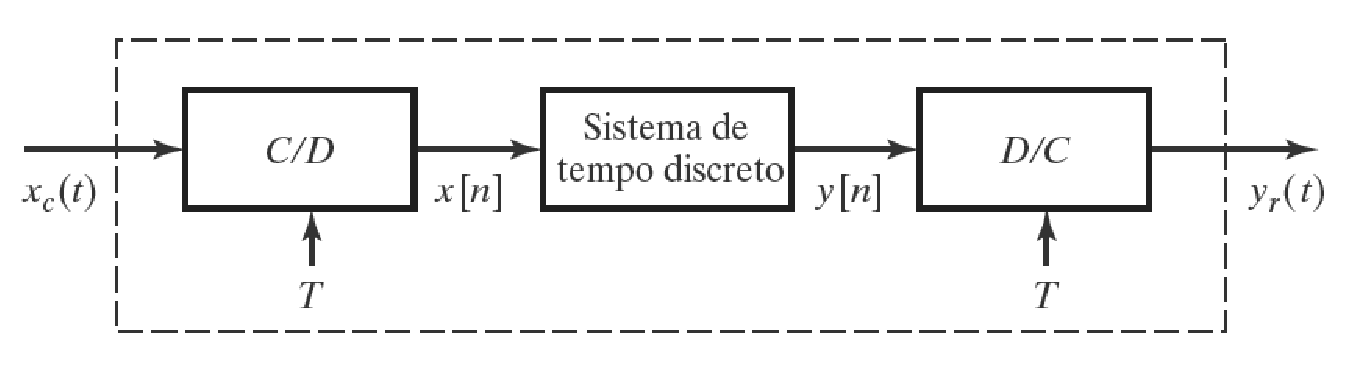
\includegraphics[width=0.9\textwidth]{figs/procdiscreto.eps}
   \end{figure}
\end{itemize}
\end{slide}

\begin{slide}{Proc. discreto de sinais cont\'inuos}
\begin{itemize}
   \item Filtro efetivo
   \begin{align}
      Y(e^{j\omega}) &= H(e^{j\omega}) X(e^{j\omega})\\
      Y_r(j\Omega)   &= H_r(j\Omega)Y(e^{j\Omega T})\\
                     &= H_r(j\Omega)H(e^{j\Omega T}) X(e^{j\Omega T})\\
                     &= H_r(j\Omega)H(e^{j\Omega T})\frac{1}{T}\sum_{k=-\infty}^{\infty}X_c(j(\Omega-k\Omega_s))\\
                     &= \begin{cases} H(e^{j\Omega T}) X_c(j\Omega), & |\Omega|<\pi /T \\
                                      0,                             & |\Omega|\geq\pi /T
                        \end{cases}
   \end{align}
\end{itemize}
\end{slide}

\begin{slide}{Proc. discreto de sinais cont\'inuos}
\begin{itemize}
   \item Filtro efetivo
   \begin{align}
      Y_r(j\Omega)   &= H_{eff}(j\Omega)X_c(j\Omega)\\
      H_{eff}        &= \begin{cases} H(e^{j\Omega T}), & |\Omega|<\pi /T \\
                                      0,                & |\Omega|\geq\pi /T
                        \end{cases}
   \end{align}
   \item Ex.: Considerando um filtro discreto do tipo passa-banda ideal com frequ\^encias de corte $\omega_{c1}=\pi/4$ e $\omega_{c2}=3\pi/4$, esboce o filtro equivalente para um sistema discreto para processamento de sinais cont\'inuos cuja frequ\^encia de amostragem \'e de $8$kHz. 
\end{itemize}
\end{slide}

\begin{slide}{Proc. digital de sinais anal\'ogicos}
 \begin{figure}
      \centering
      %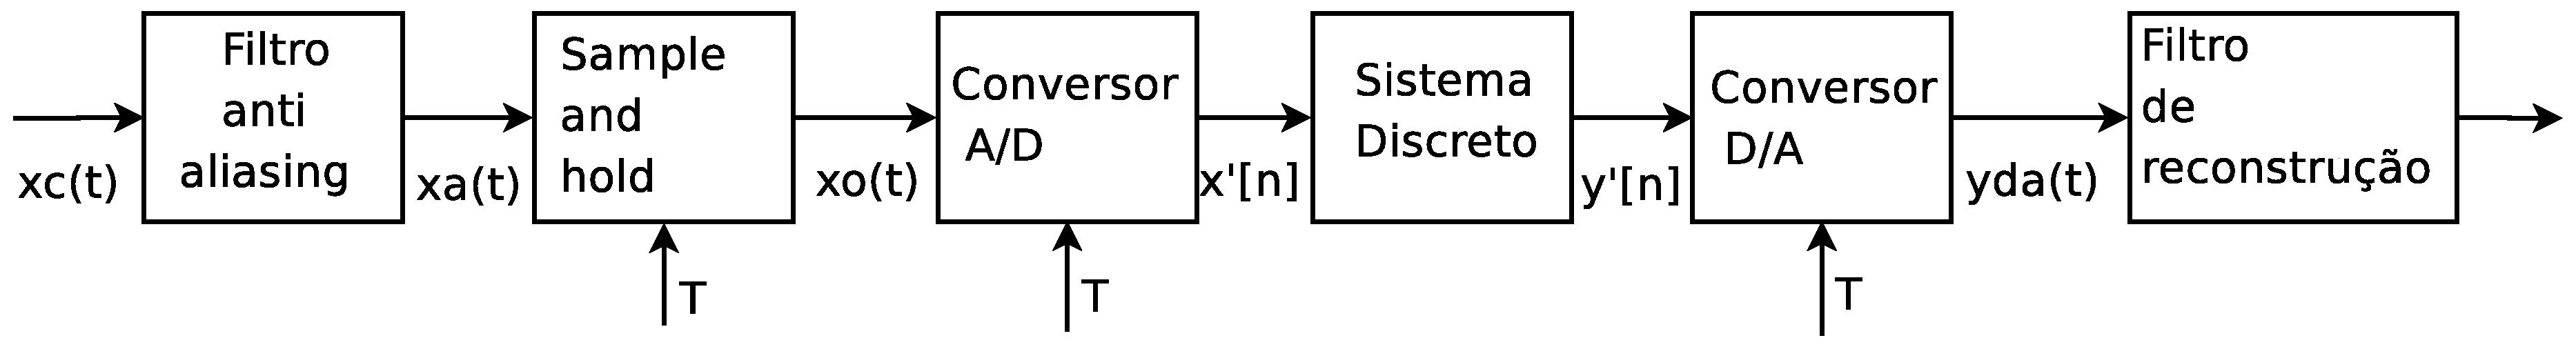
\includegraphics[width=0.9\textwidth]{figs/diagrama_completo.eps}
   \end{figure}
\begin{itemize}
   \item Pré-filtragem para evitar superposição
   \begin{itemize}
      \item Garantir o atendimento ao Teorema da Amostragem
      \begin{equation}
         H_{aa}(j\Omega) = \begin{cases}1, & |\Omega|<\Omega_c\leq \pi/T \\ 0, & |\Omega|>\Omega_c                          \end{cases}
      \end{equation}
   \end{itemize}
\end{itemize}
\end{slide}

\section{Processamento digital de sinais analógicos}
\begin{slide}{Proc. digital de sinais anal\'ogicos}
\begin{itemize}
 \item Pré-filtragem para evitar superposição
   \begin{itemize}
      \item Filtro efetivo completo
      \begin{equation}
         H_{eff}(j\Omega) = \begin{cases}H(e^{j\Omega T}), & |\Omega|<\Omega_c\\ 0, & |\Omega|>\Omega_c                          \end{cases}
      \end{equation}
      \begin{equation}
         H_{eff}(j\Omega) \approx H_{aa}(j\Omega) H(e^{j\Omega T})
      \end{equation}
      %\item Filtros analógicos seletivos em geral apresentam alto custo
   \end{itemize}
\end{itemize}
\end{slide}

%\begin{slide}{Proc. digital de sinais anal\'ogicos}
%\begin{itemize}
% \item Pré-filtragem para evitar superposição
%   \begin{itemize}
%      \item Alternativa usando \emph{down sampling}
%      \begin{figure}
%          \centering
%          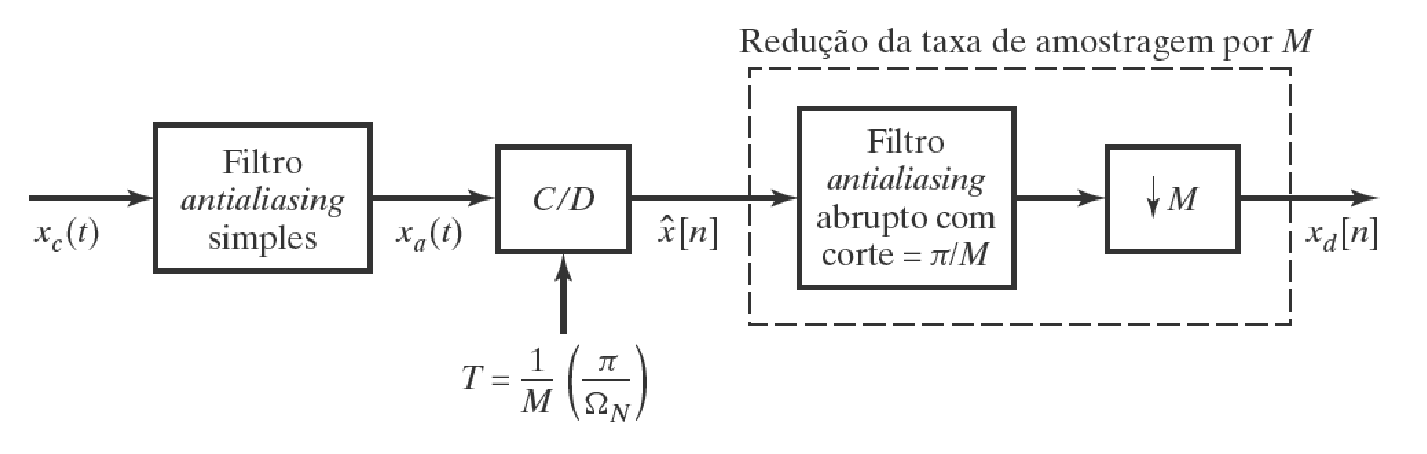
\includegraphics[width = 0.9\textwidth]{figs/aa_alt.eps}
%      \end{figure}
%   \end{itemize}
%\end{itemize}
%\end{slide}

%\begin{slide}{Proc. digital de sinais anal\'ogicos}
%\begin{itemize}
% \item Pré-filtragem para evitar superposição
%   \begin{itemize}
%      \item Alternativa usando \emph{down sampling} (efeitos na frequência)
%      \begin{figure}
%          \centering
%          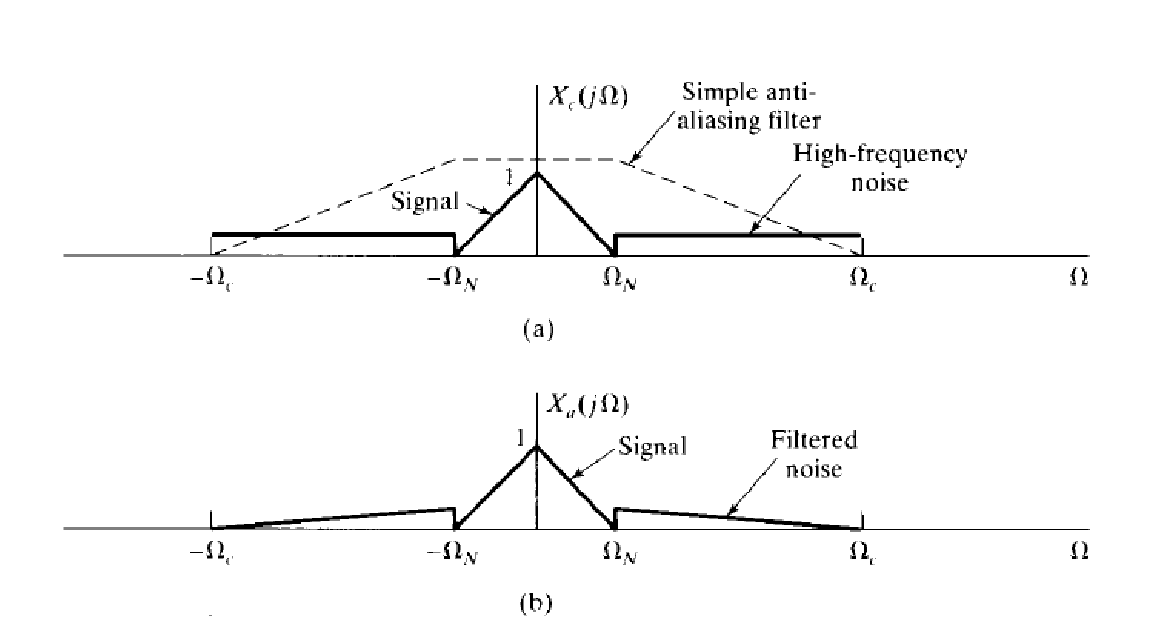
\includegraphics[width = 0.9\textwidth]{figs/aa_alt_freq1.eps}
%      \end{figure}
%   \end{itemize}
%\end{itemize}
%\end{slide}

%\begin{slide}{Proc. digital de sinais anal\'ogicos}
%\begin{itemize}
% \item Pré-filtragem para evitar superposição
%   \begin{itemize}
%      \item Alternativa usando \emph{down sampling} (efeitos na frequência)
%      \begin{figure}
%          \centering
%          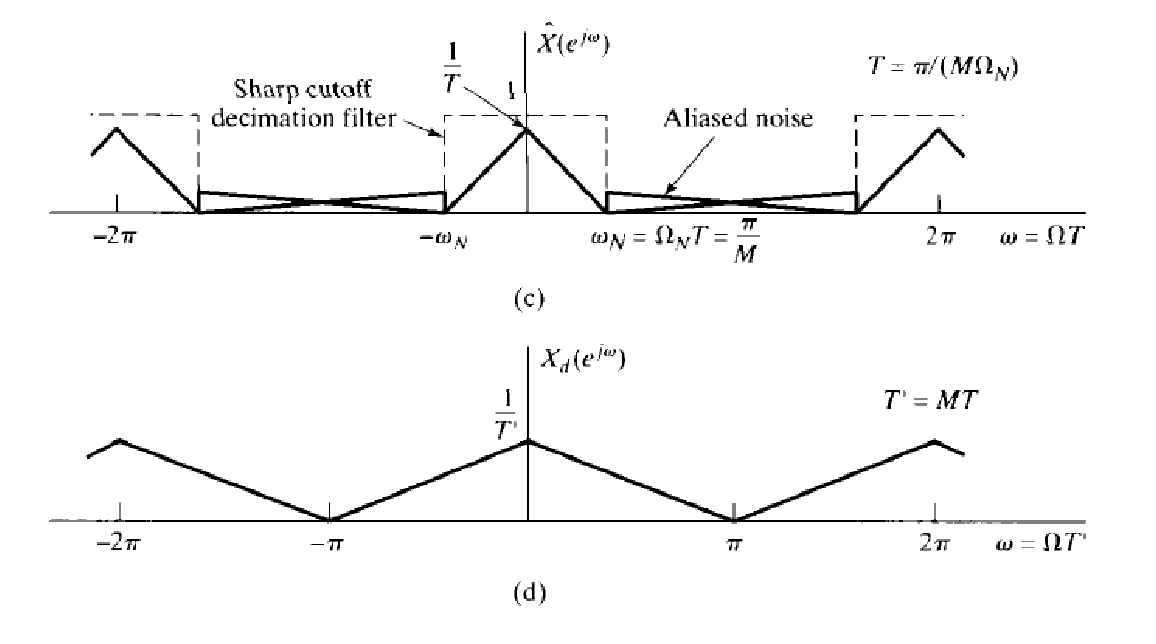
\includegraphics[width = 0.9\textwidth]{figs/aa_alt_freq2.eps}
%      \end{figure}
%   \end{itemize}
%\end{itemize}
%\end{slide}

\begin{slide}{Proc. digital de sinais anal\'ogicos}
\begin{itemize}
   \item Conversão analógico-digital
   \begin{itemize}
      \item Amostragem e retenção (\emph{sample and hold})
      \begin{figure}
         \centering
          %\includegraphics[width = 0.4\textwidth]{figs/ad_conv1.eps}
          %\includegraphics[width = 0.4\textwidth]{figs/ad_conv2.eps}
      \end{figure}

   \end{itemize}
   %\item Análise dos erros de quantização
   %\item Conversão digital-analógica
   %\item 
\end{itemize}
\end{slide}

\begin{slide}{Proc. digital de sinais anal\'ogicos}
\begin{itemize}
   \item Conversão analógico-digital
   \begin{itemize}
      \item Amostragem e retenção (\emph{sample and hold})
      \begin{equation}
          h_0(t) = \begin{cases} 1, & 0<t<T\\0, & \text{outro intervalo}\end{cases}
      \end{equation}
      \begin{equation}
          x_0(t) = h_0(t)\ast x_s(t)
      \end{equation}
      %\begin{figure}
       %  \centering
        %  \includegraphics[width = 0.5\textwidth]{ad_conv1.eps}
         % \includegraphics[width = 0.5\textwidth]{ad_conv2.eps}
      %\end{figure}
   \end{itemize}
   %\item Análise dos erros de quantização
   %\item Conversão digital-analógica
   %\item 
\end{itemize}
\end{slide}

\begin{slide}{Proc. digital de sinais anal\'ogicos}
\begin{itemize}
   \item Conversão analógico-digital
   \begin{itemize}
      \item Amostragem e retenção (\emph{sample and hold})
      \begin{figure}
        \centering
         %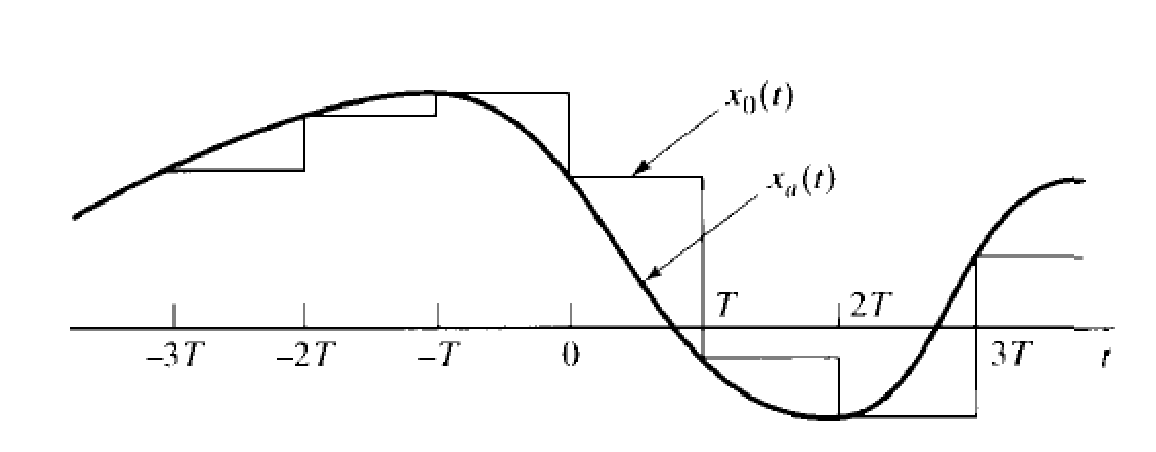
\includegraphics[width = 0.8\textwidth]{figs/ad_conv3.eps}
        %\includegraphics[width = 0.5\textwidth]{ad_conv2.eps}
      \end{figure}

   \end{itemize}
   %\item Análise dos erros de quantização
   %\item Conversão digital-analógica
   %\item 
\end{itemize}
\end{slide}

\begin{slide}{Proc. digital de sinais anal\'ogicos}
\begin{itemize}
   \item Conversão analógico-digital
   \begin{itemize}
      \item Quantização 
      \begin{figure}
        \centering
         %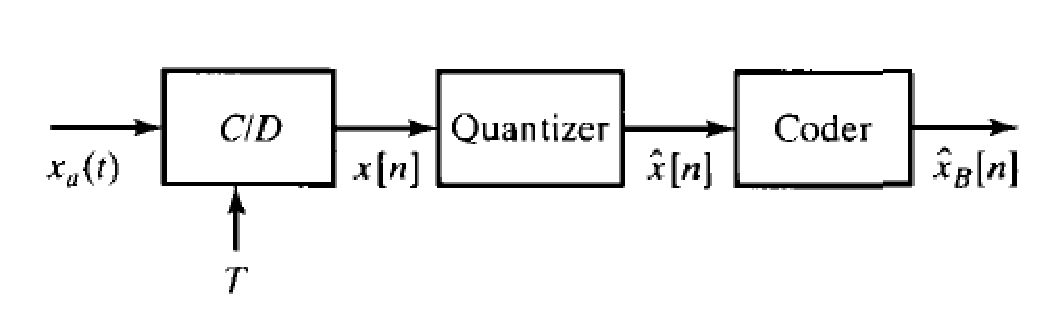
\includegraphics[width = 0.8\textwidth]{figs/ad_conv4.eps}
        %\includegraphics[width = 0.5\textwidth]{ad_conv2.eps}
      \end{figure}
\begin{equation}
          \hat x[n] = Q(x[n])
      \end{equation}
   \end{itemize}
   %\item Análise dos erros de quantização
   %\item Conversão digital-analógica
   %\item 
\end{itemize}
\end{slide}

\begin{slide}{Proc. digital de sinais anal\'ogicos}
\begin{itemize}
   \item Conversão analógico-digital
   \begin{itemize}
      \item Quantização 
      \begin{figure}
        \centering
         %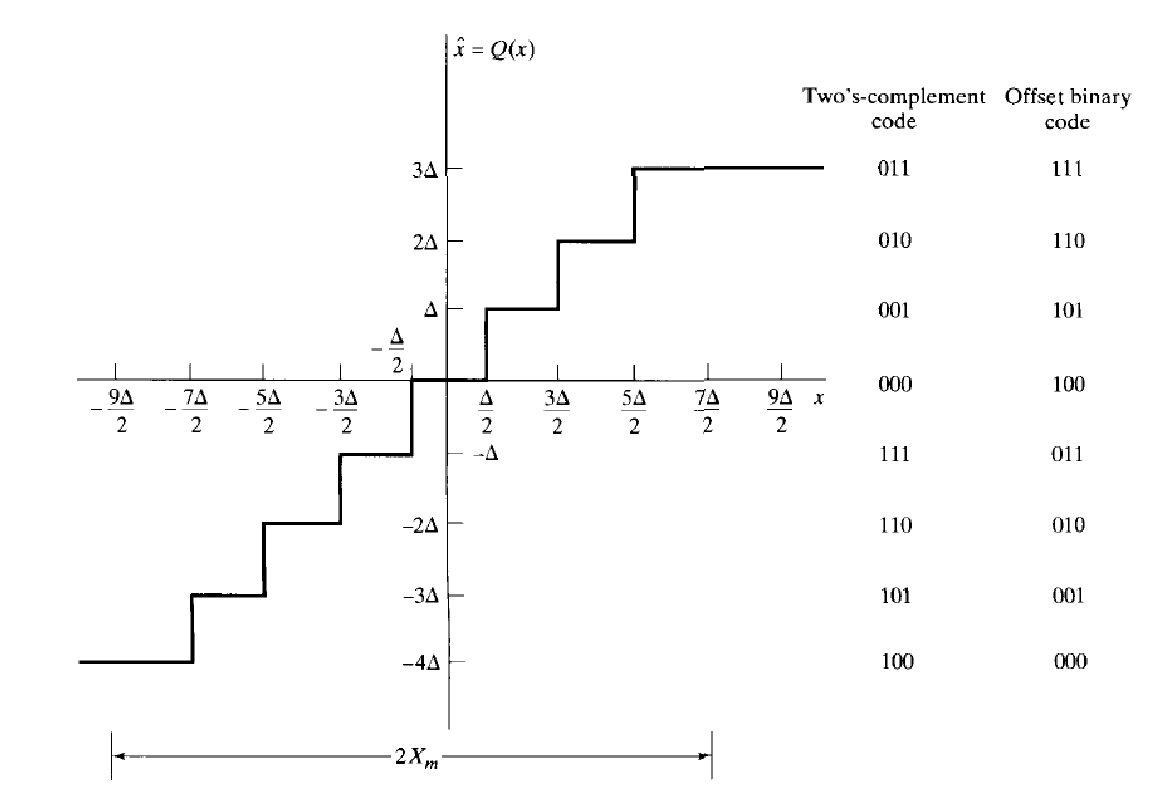
\includegraphics[width = 0.65\textwidth]{figs/ad_quantz.eps}
        %\includegraphics[width = 0.5\textwidth]{ad_conv2.eps}
      \end{figure}

   \end{itemize}
   %\item Análise dos erros de quantização
   %\item Conversão digital-analógica
   %\item 
\end{itemize}
\end{slide}


\begin{slide}{Proc. digital de sinais anal\'ogicos}
\begin{itemize}
   \item Conversão analógico-digital
   \begin{itemize}
      \item Quantização 
      \begin{figure}
        \centering
         %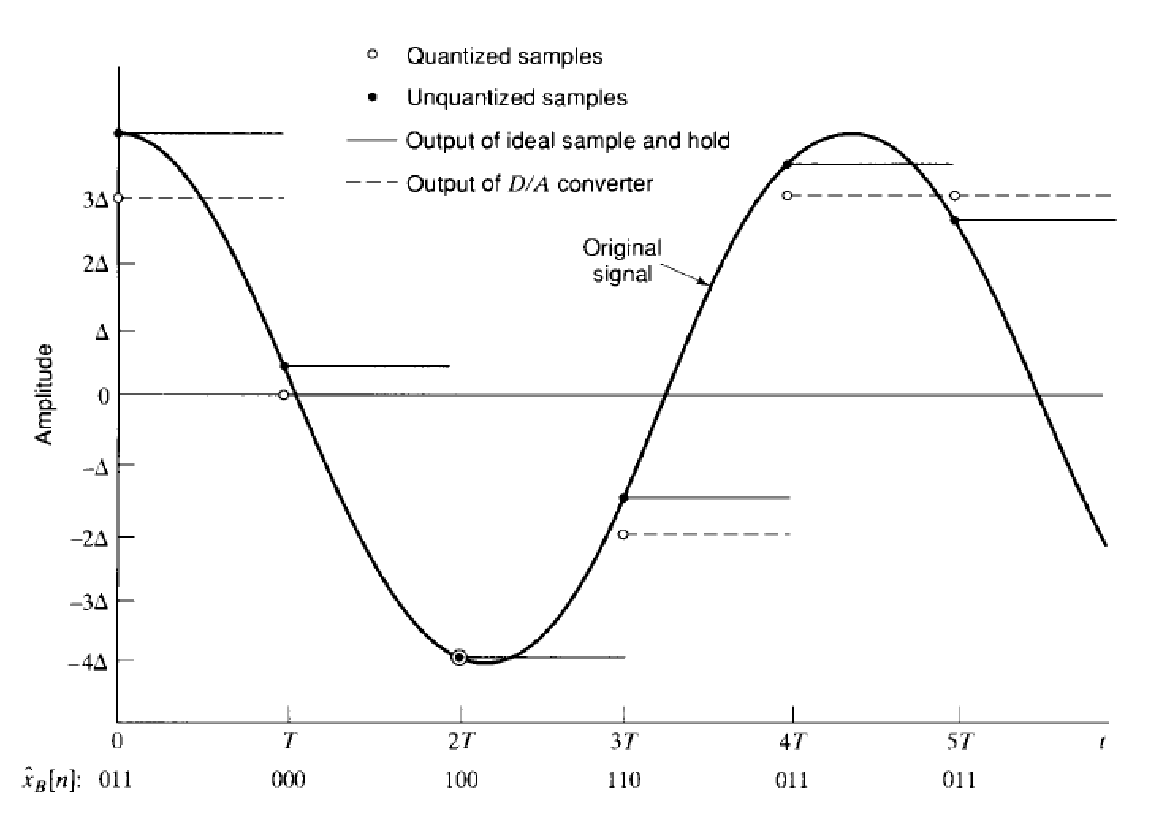
\includegraphics[width = 0.65\textwidth]{figs/ad_quantz2.eps}
        %\includegraphics[width = 0.5\textwidth]{ad_conv2.eps}
      \end{figure}

   \end{itemize}
   %\item Análise dos erros de quantização
   %\item Conversão digital-analógica
   %\item 
\end{itemize}
\end{slide}

\begin{slide}{Proc. digital de sinais anal\'ogicos}
\begin{itemize}
   \item Conversão analógico-digital
   \begin{itemize}
      \item Análise do erro de quantização
      \begin{equation}
        e[n] = \hat x[n] - x[n]
      \end{equation}

        \begin{equation}
         -\frac{\Delta}{2}<e[n]\leq \frac{\Delta}{2}
        \end{equation}

        \begin{equation}
         \left (-X_m-\frac{\Delta}{2}\right )<x[n]\leq \left (X_m-\frac{\Delta}{2}\right )
        \end{equation}


      %\item Considerações sobre $e[n]$:

   \end{itemize}
   %\item 
   %\item Conversão digital-analógica
   %\item 
\end{itemize}
\end{slide}

\begin{slide}{Proc. digital de sinais anal\'ogicos}
\begin{itemize}
   \item Conversão analógico-digital
   \begin{itemize}
      \item Análise do erro de quantização
      \begin{itemize}
         \item Considerações sobre $e[n]$:
         \begin{itemize}
             \item $e[n]$: amostras de um processo aleatório estacionário;
             \item $e[n]$ e $x[n]$ são não-correlacionados;
             \item $e[n]$ é ruído do tipo branco;
             \item $e[n]$ possui distribuição uniforme entre $-\Delta /2$ e $\Delta /2$
         \end{itemize}
         \textcolor{red}{Tarefa: Calcule a média e a variância de $e[n]$.}
      \end{itemize}

   \end{itemize}
   %\item 
   %\item Conversão digital-analógica
   %\item 
\end{itemize}
\end{slide}
\begin{slide}{Proc. digital de sinais anal\'ogicos}
\begin{itemize}
   \item Conversão analógico-digital
   \begin{itemize}
      \item Análise do erro de quantização
       \begin{equation}
        \sigma^2_e = \frac{\Delta^2}{12} = \frac{2^{-2B}X_m^2}{12}
      \end{equation}
      Razão Sinal-Ruído:
     \begin{align*}
         SNR &= 10\log_{10}\left ( \frac{\sigma_x^2}{\sigma_e^2} \right )= 10\log_{10}\left ( \frac{12\cdot 2^{2B}\sigma_x^2}{X_m^2} \right )\\
                 &= 6,02 B + 10,8-20\log_{10}\left(\frac{X_m}{\sigma_x} \right )
     \end{align*}


   \end{itemize}
   %\item 
   %\item Conversão digital-analógica
   %\item 
\end{itemize}
\end{slide}


\begin{slide}{Proc. digital de sinais anal\'ogicos}
\begin{itemize}
   \item Conversão digital-analógica
   \begin{itemize}
      \item Filtro de restauração 
      \begin{figure}
        \centering
         %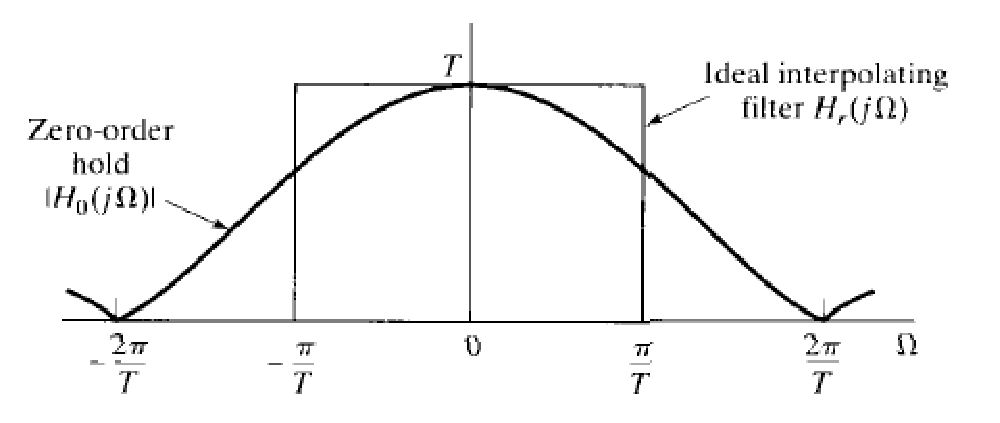
\includegraphics[width = 0.45\textwidth]{figs/da_conv1.eps}
        %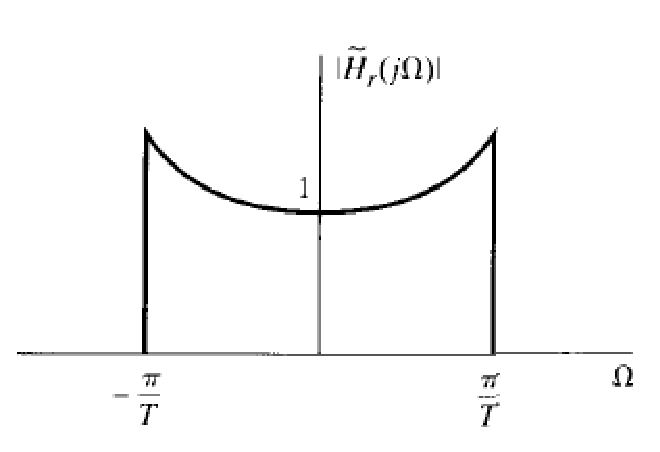
\includegraphics[width = 0.45\textwidth]{figs/da_conv2.eps}
      \end{figure}

   \end{itemize}
   %\item Análise dos erros de quantização
   %\item 
   %\item 
\end{itemize}
\end{slide}

\section{Mudança de taxa de amostragem usando processamento discreto}
\begin{slide}{Mudança de taxa de amostragem}
	\begin{itemize}
		\item Objetivo: obtenção de um novo sinal discreto com taxa de amostragem diferente da usada inicialmente
			\begin{equation*}
				x_1[n] = x_c(nT_1)
			\end{equation*}
		\item Possível solução: reconstrução a partir de $x[n]$ e nova amostragem usando $T_1$
		\begin{itemize}
			\item Problemas na prática: uso de elementos  de conversão não ideais (ADC e DAC)
		\end{itemize}
		\item Outra solução: mudança de taxa no domínio discreto, a partir de $x[n]$
		\begin{itemize}
			\item Redução por fatores inteiros
			\item Aumento por fatores inteiros
			\item Mudança por fatores não inteiros
		\end{itemize}
	\end{itemize}
\end{slide}

\begin{slide}{Redução da taxa de amostragem por fatores inteiros}
	\begin{itemize}
		\item Downsampling
			\begin{equation*}
				x_d[n] = x[nM] = x_c(nMT)
			\end{equation*}
			onde $M \in Z$
		\item Domínio espectral
			\begin{align*}
     				X(e^{j\omega})& = \frac{1}{T}\sum_{k=-\infty}^{\infty}X_c\left(j\left(\frac{\omega}{T}-\frac{2k\pi}{T}\right )\right )\\
				X_d(e^{j\omega})& = \frac{1}{MT}\sum_{r=-\infty}^{\infty}X_c\left(j\left(\frac{\omega}{MT}-\frac{2r\pi}{MT}\right )\right )
			\end{align*}
	\end{itemize}
\end{slide}

\begin{slide}{Redução da taxa de amostragem por fatores inteiros}
	\begin{itemize}
		\item Fazendo uma mudança de variável $ r = i + kM$
			\begin{align*}
				X_d(e^{j\omega})& = \frac{1}{M}\sum_{i=0}^{M-1}\left \{\frac{1}{T}\sum_{k=-\infty}^{\infty}X_c\left(j\left(\frac{\omega}{MT}-\frac{2k\pi}{T}-\frac{2i\pi}{MT}\right )\right )\right \}\\
				& = \frac{1}{M}\sum_{i=0}^{M-1}X\left (e^{j\left (\frac{\omega}{M}-\frac{2i\pi}{M}\right )}\right )
			\end{align*}
			\begin{itemize}
				\item Comparar com a expressão para $X(e^{j\omega})$.
				\item Para que não ocorra \emph{aliasing} no processo de reamostragem, $X(e^{j\omega})$ deve ser limitado em banda
					\begin{equation*}
						X(e^{j\omega})= 0, \qquad \omega_N \leq |\omega| \leq \pi
					\end{equation*}
					e  $2\pi/M \geq 2 \omega_N$
			\end{itemize}
	\end{itemize}
\end{slide}

\begin{slide}{Redução da taxa de amostragem por fatores inteiros - Exemplo}
	\begin{itemize}
		\item Exemplo para $M=2$
			\begin{itemize}
				\item Espectro do sinal contínuo original
			\begin{figure}
				\centering
				%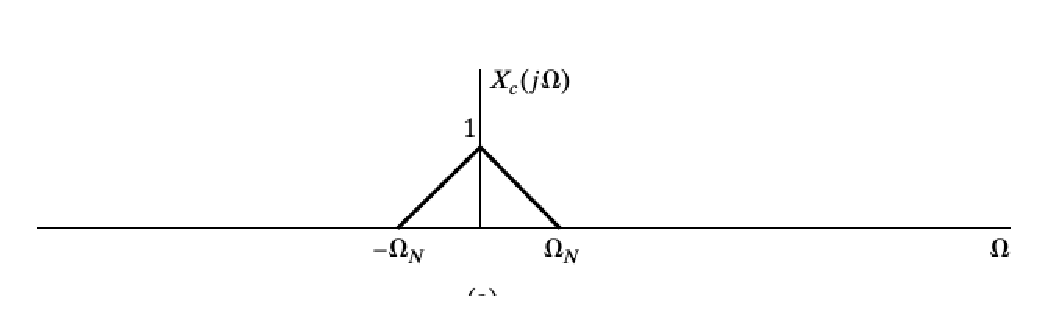
\includegraphics[width=0.45\textwidth]{figs/4-20a.eps}
		        \end{figure}
		\item Espectros para a primeira amostragem 
			\begin{figure}
				\centering
				%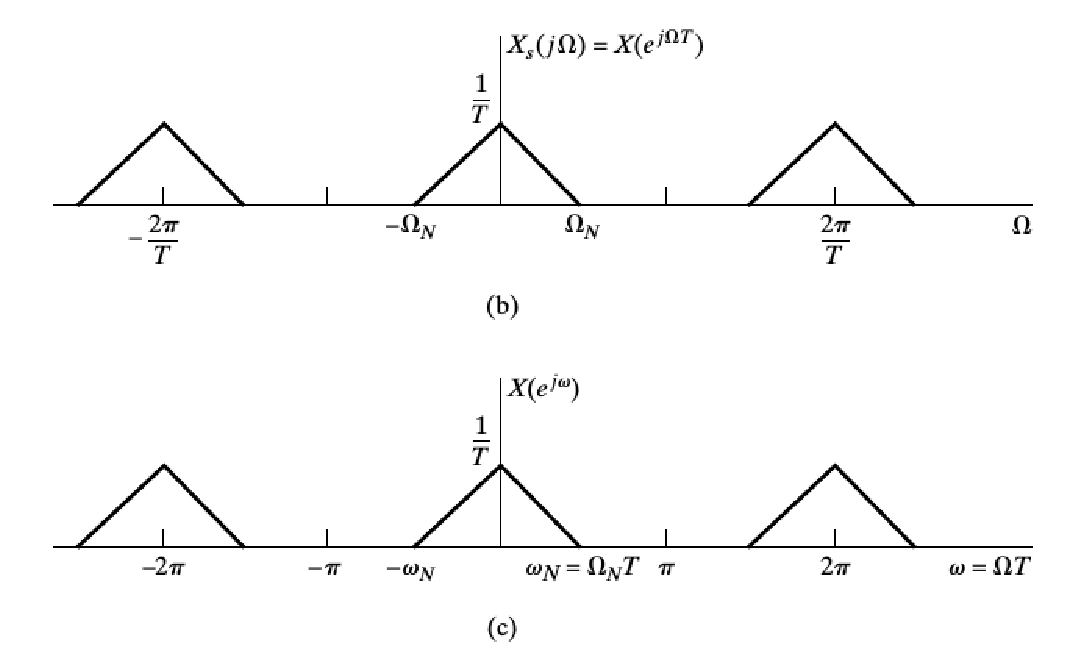
\includegraphics[width=0.45\textwidth]{figs/4-20bc.eps}
		        \end{figure}
			\end{itemize}
	\end{itemize}
\end{slide}

\begin{slide}{Redução da taxa de amostragem por fatores inteiros - Exemplo}
	\begin{itemize}
		\item Exemplo para $M=2$
			\begin{itemize}
		\item Espectros após a redução de taxa de amostragem 
			\begin{figure}
				\centering
				%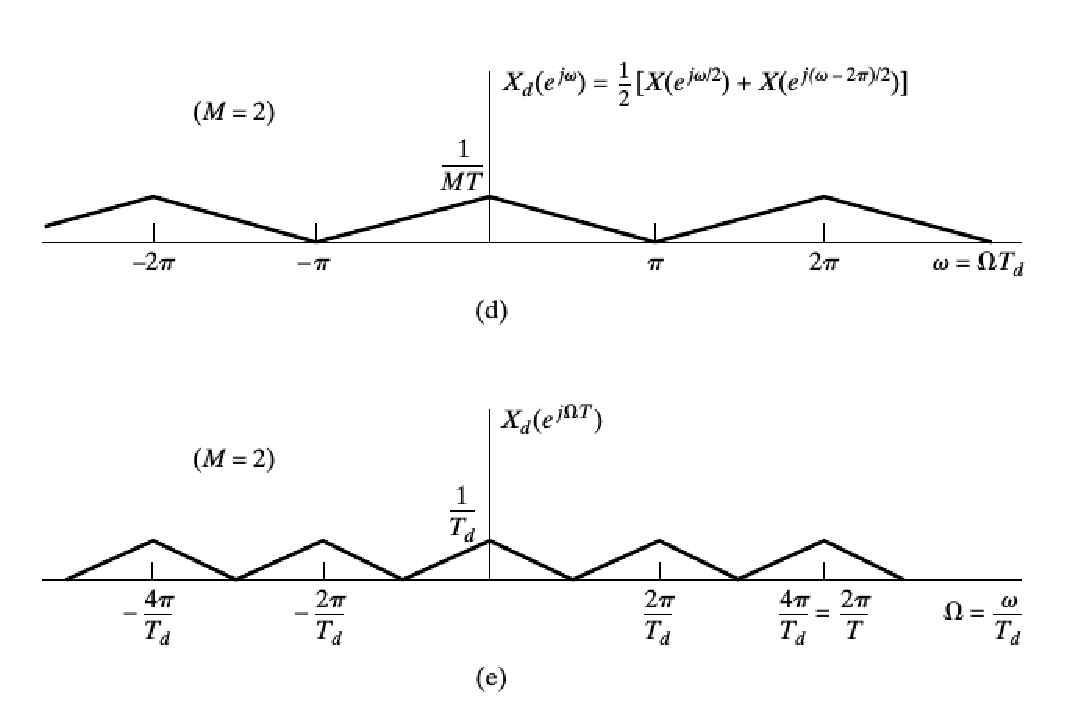
\includegraphics[width=0.65\textwidth]{figs/4-20de.eps}
		        \end{figure}
			\end{itemize}
	\end{itemize}
\end{slide} 

\begin{slide}{Redução da taxa de amostragem por fatores inteiros - Exemplo}
	\begin{itemize}
		\item Exemplo para $M=3$
			\begin{itemize}
		\item Espectro após a redução de taxa de amostragem e filtro anti-aliasing
			\begin{figure}
				\centering
				%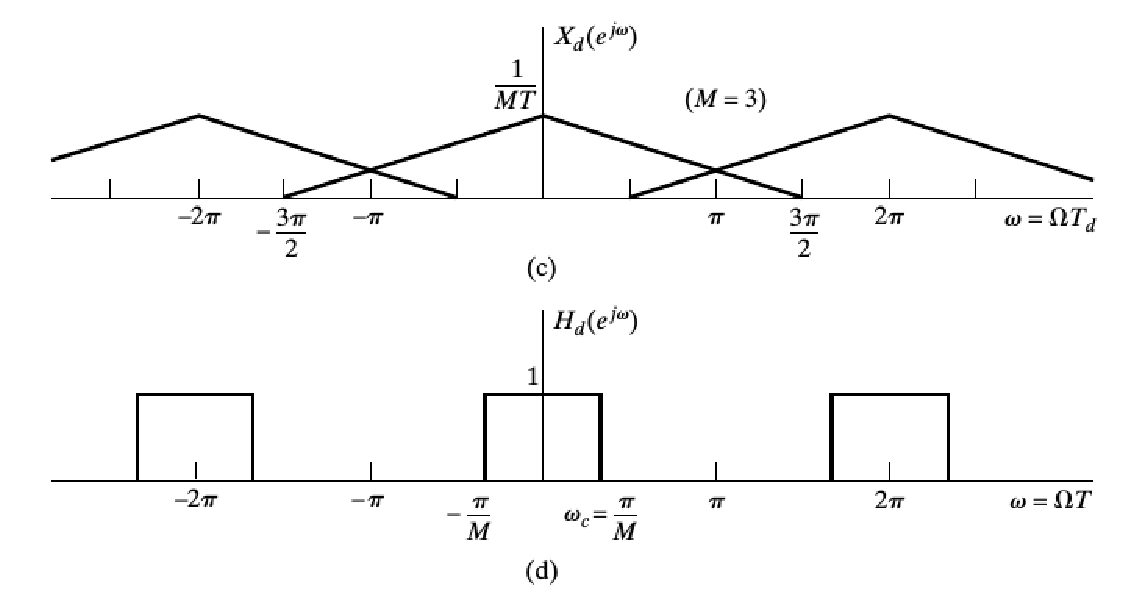
\includegraphics[width=0.8\textwidth]{figs/4-21cd.eps}
		        \end{figure}
			\end{itemize}
	\end{itemize}
\end{slide}
\begin{slide}{Redução da taxa de amostragem por fatores inteiros - Exemplo}
	\begin{itemize}
		\item Exemplo para $M=3$
			\begin{itemize}
		\item Espectro após a redução de taxa de amostragem após filtragem anti-aliasing
			\begin{figure}
				\centering
				%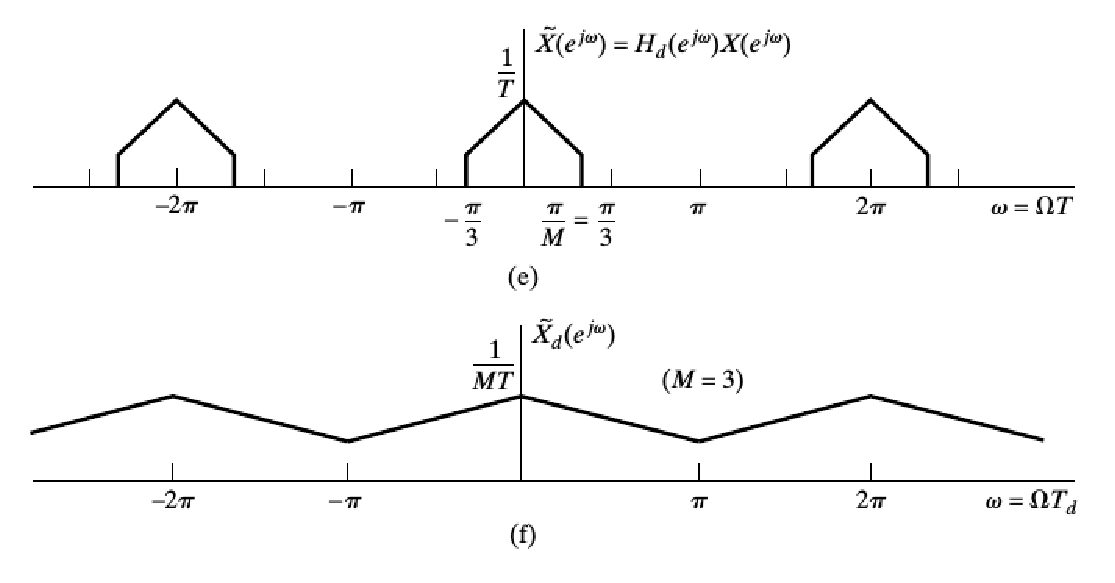
\includegraphics[width=0.8\textwidth]{figs/4-21ef.eps}
		        \end{figure}
			\end{itemize}
	\end{itemize}
\end{slide}
\begin{slide}{Redução da taxa de amostragem por fatores inteiros}
	\begin{itemize}
		\item Sistema geral
			\begin{itemize}
				\item A redução de taxa de amostragem é precedida por filtragem passa-baixas para evitar o \emph{aliasing}
				\begin{figure}
					\centering
					%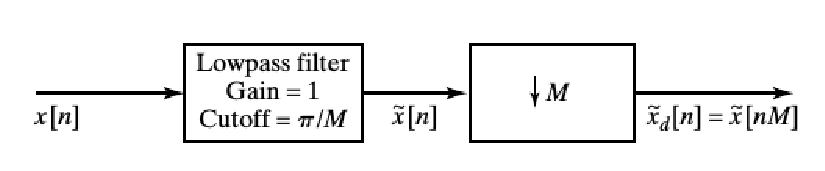
\includegraphics[width=0.8\textwidth]{figs/4-22.eps}
		        	\end{figure}
			\end{itemize}
	\end{itemize}
\end{slide}

%%%%
\begin{slide}{Aumento da taxa de amostragem por fatores inteiros}
	\begin{itemize}
		\item Objetivo: obter uma sequência $x_i[n]$ que seja equivalente à amostragem de $x_c(t)$ usando um período de amostragem $L$ vezes menor que $T$, a partir da sequência $x[n]$, ou seja 
			\begin{equation*}
				x_i[n] = x_c(nT/L)
			\end{equation*}
			onde $L \in Z$ e 
			\begin{equation*}
				x[n] = x_c(nT)
			\end{equation*}
		\item Pelas expressões acima:
			\begin{equation*}
				x_i[n] = x[n/L] = x_c(nT/L), \qquad n= 0, \pm L, \pm 2L, \dots
			\end{equation*}
	\end{itemize}
\end{slide}

\begin{slide}{Aumento da taxa de amostragem por fatores inteiros}
	\begin{itemize}
		\item Expansor de taxa de amostragem 
			\begin{align*}
				x_e[n] &= 
				\begin{cases}
					x[n/L],  & n= 0, \pm L, \pm 2L, \dots\\
					0, &\text{outro valor}
				\end{cases}\\
				&= \sum_{k=-\infty}^{\infty}x[k]\delta[n-kL]
			\end{align*}
		\item No domínio da frequência:
			\begin{align*}
				X_e(e^{j\omega})& = \sum_{n=-\infty}^{\infty}\left ( \sum_{k=-\infty}^{\infty}x[k]\delta[n-kL] \right ) e^{-j\omega n}\\
				 &=  \sum_{k=-\infty}^{\infty}x[k] e^{-j\omega L k}\\
				 &=  X(e^{j\omega L})
			\end{align*}
	\end{itemize}
\end{slide}

\begin{slide}{Aumento da taxa de amostragem por fatores inteiros - Exemplo}
	\begin{itemize}
		\item Exemplo para $L=2$
			\begin{itemize}
				\item Espectro do sinal contínuo original
			\begin{figure}
				\centering
				%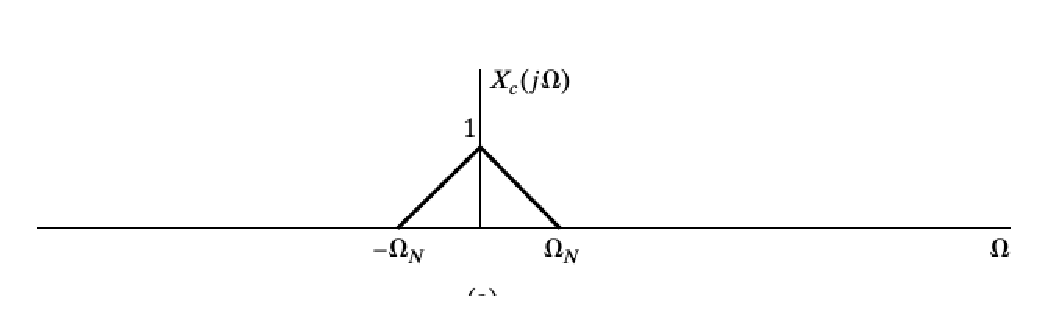
\includegraphics[width=0.4\textwidth]{figs/4-20a.eps}
		        \end{figure}
		\item Espectros para a primeira amostragem e após expansor
			\begin{figure}
				\centering
				%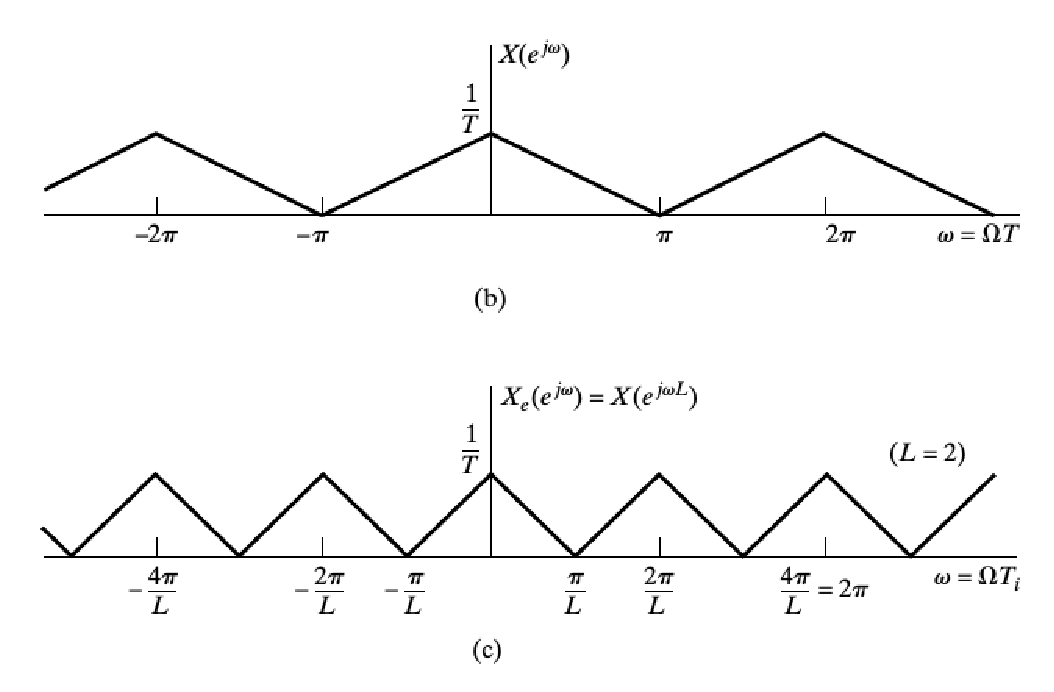
\includegraphics[width=0.4\textwidth]{figs/4-24bc.eps}
		        \end{figure}
			\end{itemize}
	\end{itemize}
\end{slide}

\begin{slide}{Aumento da taxa de amostragem por fatores inteiros - Exemplo}
	\begin{itemize}
		\item Exemplo para $L=2$
			\begin{itemize}
		\item Filtro de reconstrução e espectro final 
			\begin{figure}
				\centering
				%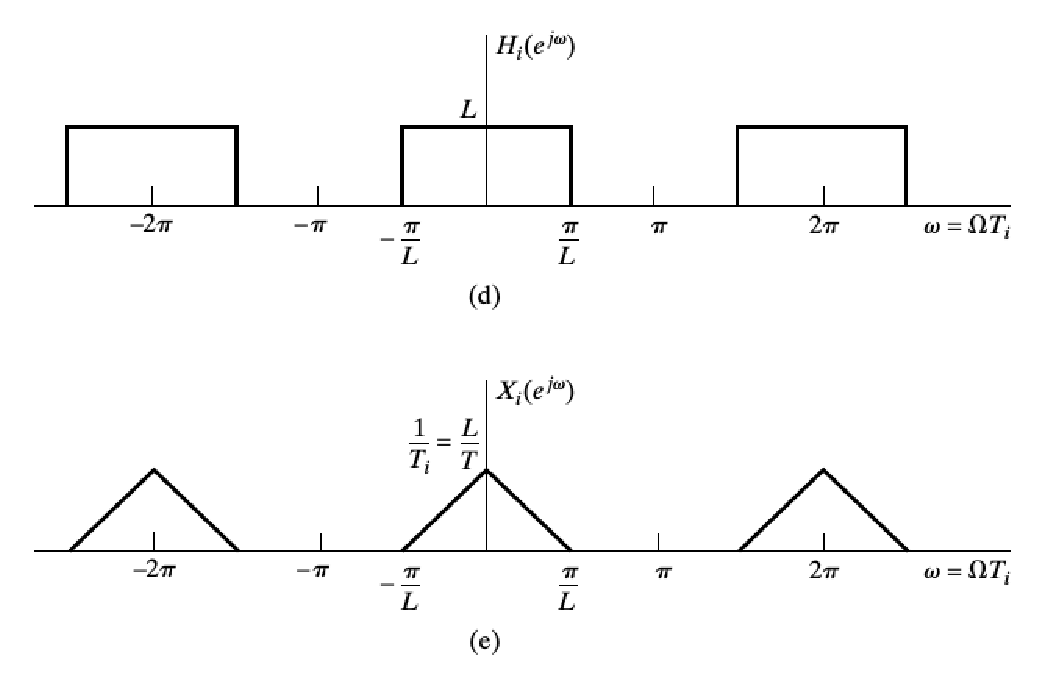
\includegraphics[width=0.65\textwidth]{figs/4-24de.eps}
		        \end{figure}
			\end{itemize}
	\end{itemize}
\end{slide} 
\begin{slide}{Aumento da taxa de amostragem por fatores inteiros}
	\begin{itemize}
		\item Sistema geral (\emph{upsampling}, interpolador) 
			\begin{figure}
				\centering
				%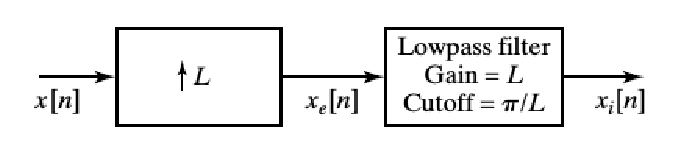
\includegraphics[width=0.8\textwidth]{figs/4-23.eps}
		        \end{figure}
	\end{itemize}
\end{slide} 

\begin{slide}{Aumento da taxa de amostragem por fatores inteiros }
	\begin{itemize}
		\item Interpolador ideal
			\begin{equation*}
				h_\text{i}[n] = \frac{\sin (\pi n/L)}{\pi n/L}
			\end{equation*}
		\item Interpolador linear
			\begin{equation*}
				h_\text{lin}[n] = \begin{cases} 1-|n|/L, & |n|\leq L\\ 0, & \text{outro caso} \end{cases}
			\end{equation*}
			\begin{figure}
				\centering
				%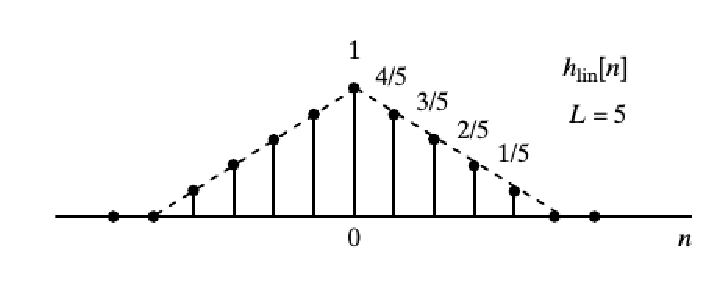
\includegraphics[width=0.6\textwidth]{figs/4-25.eps}
		        \end{figure}
	\end{itemize}
\end{slide}
\begin{slide}{Aumento da taxa de amostragem por fatores inteiros }
	\begin{itemize}
		\item Interpolador linear -- determinação da saída
			\begin{equation*}
				x_\text{lin}[n]=x_e[n]*h_\text{lin}[n]
			\end{equation*}
			\begin{figure}
				\centering
				%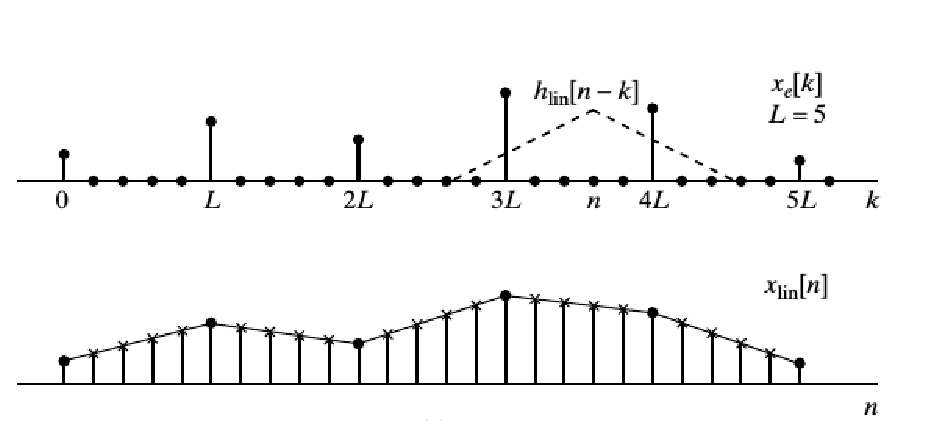
\includegraphics[width=0.4\textwidth]{figs/4-26a.eps}
		        \end{figure}
		\item Comparação no domínio da frequência 
			\begin{figure}
				\centering
				%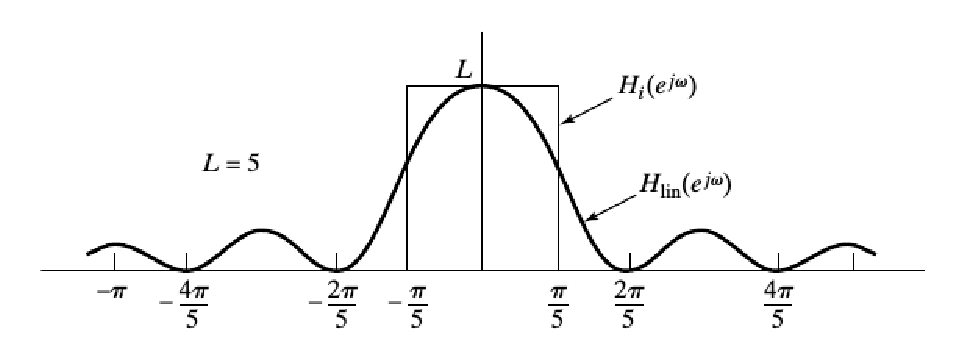
\includegraphics[width=0.4\textwidth]{figs/4-26b.eps}
		        \end{figure}
	\end{itemize}
\end{slide}
\begin{slide}{Aumento da taxa de amostragem por fatores inteiros}
	\begin{itemize}
		\item Características gerais de um interpolador
			\begin{align*}
				\tilde h_i[n]&= 0, \qquad |n|\geq KL\\
				\tilde h_i[n]&= \tilde h_i[-n], \qquad |n|\leq KL\\
				\tilde h_i[n]&= 1, \qquad n=0\\
				\tilde h_i[n]&= 0, \qquad n=\pm L, \pm 2L,\dots, \pm KL
			\end{align*}
		\item Sinal interpolado
			\begin{align*}
				\tilde x_i[n] &= x_e[n] * \tilde h_i[n]\\
				              &= \sum_{k= n-KL+1}^{n+KL-1} x_e[k]\tilde h_i[n-k]
			\end{align*}
	\end{itemize}
\end{slide}
\begin{slide}{Aumento da taxa de amostragem por fatores inteiros}
	\begin{itemize}
		\item Pesquisar dois outros interpoladores.
		\item Especificar suas respostas ao impulso
		\item Determinar suas respostas em frequência
		\item Comparar com o interpolador linear
	\end{itemize}
\end{slide}

%%%%
\begin{slide}{Mudança da taxa de amostragem por fatores não-inteiros}
	\begin{itemize}
		\item Objetivo: obter $\tilde x_d[n]$, a partir de $x[n]$, tal que 
			\begin{equation*}
				\tilde x_d[n] = x_c(nMT/L)
			\end{equation*}
			onde $L, M \in Z$ e 
			\begin{equation*}
				x[n] = x_c(nT)
			\end{equation*}
			\begin{figure}
				\centering
				%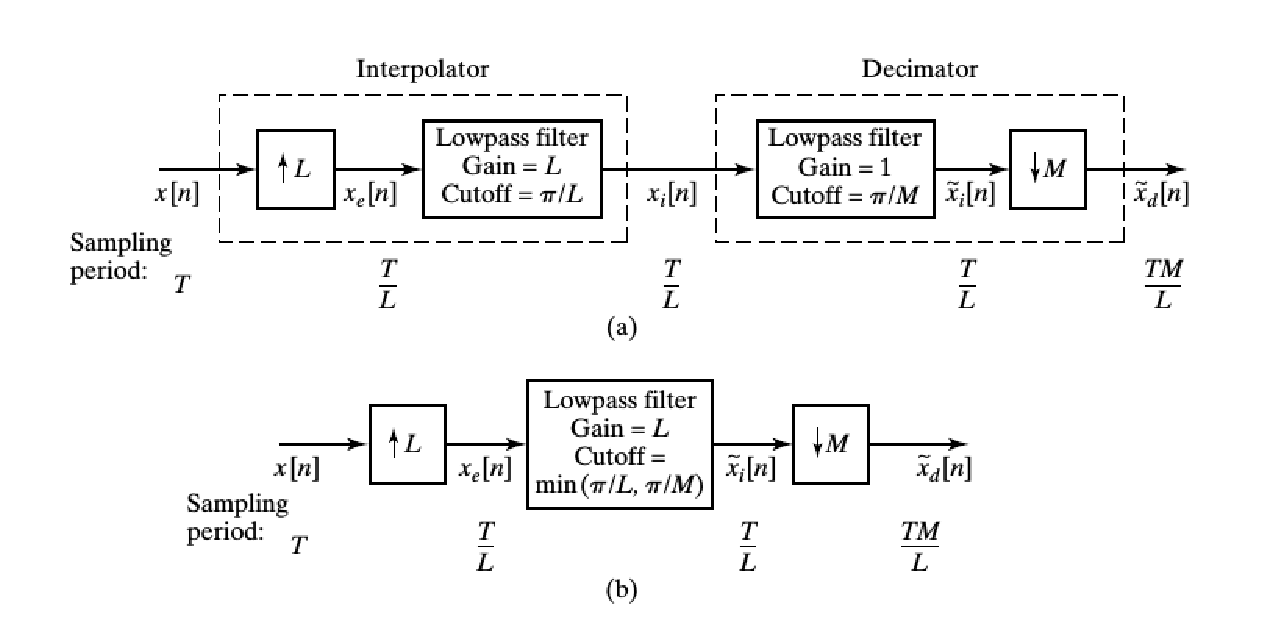
\includegraphics[width=0.6\textwidth]{figs/4-29.eps}
		        \end{figure}
	\end{itemize}
\end{slide}

%\section{Processamento de sinais multitaxa}
%\begin{slide}{Introdução}
%	\begin{itemize}
%		\item Conjunto de técnicas que usa \emph{upsampling}, \emph{downsampling}, expansores e compressores para melhorar a eficiência de sistemas de processamento de sinais
%		\item Objetivo: redução de complexidade computacional associada a operações de mudança de taxa de amostragem
%		\item Aplicações:
%			\begin{itemize}
%				\item Conversão AD e DA que fazem uso de \emph{oversampling} e \emph{noise shaping}
%				\item Banco de filtros
%				\item \emph{Wavelets}
%			\end{itemize}
%	\end{itemize}
%\end{slide}
%%%%%%%%%%
%\begin{slide}{Intercâmbio entre filtragem e compressão/expansão}
%	\begin{itemize}
%		\item Equivalência para \emph{downsampling}
%			\begin{figure}
%				\centering
%				\includegraphics[width=0.3\textwidth]{figs/4-31.eps}
%			\end{figure}
%			\begin{align*}
%				X_b(e^{j\omega}) &=H(e^{j\omega M}) X(e^{j\omega})\\
%				Y(e^{j\omega})&= \frac{1}{M} \sum_{i=0}^{M-1} X_b(e^{j(\omega/M - 2\pi i/M)})\\
%			%	&= \frac{1}{M} \sum_{i=0}^{M-1} H(e^{j\omega})X(e^{j(\omega/M - 2\pi i/M})\\
%				&= H(e^{j\omega})\frac{1}{M} \sum_{i=0}^{M-1} X(e^{j(\omega/M - 2\pi i/M)}) = H(e^{j\omega})X_a(e^{j\omega})
%			\end{align*}
%	\end{itemize}
%			
%\end{slide}
%
%\begin{slide}{Intercâmbio entre filtragem e compressão/expansão}
%	\begin{itemize}
%		\item Equivalência para \emph{upsampling}
%			\begin{figure}
%				\centering
%				\includegraphics[width=0.3\textwidth]{figs/4-32.eps}
%			\end{figure}
%			\begin{align*}
%				Y(e^{j\omega})&=X_a(e^{j\omega L})\\
%%				&=H(e^{j\omega L}) X(e^{j\omega L})\\
%				X_b(e^{j\omega})&= X(e^{j\omega L})\\
%				Y(e^{j\omega})&=H(e^{j\omega L})X_b(e^{j\omega })
%			\end{align*}
%	\end{itemize}
%			
%\end{slide}
%
%\begin{slide}{Dizimação e interpolação multiestágios}
%	\begin{itemize}
%		\item Situação: downsampling com razão $M = M_1M_2$
%		\item Problema: frequência de corte do filtro passa-baixas $\pi/(M_1M_2)$ pode resultar em filtros de comprimento muito longo
%		\item Solução: downsampling em dois estágios com frequências de corte maiores ($\pi/M_1$ e $\pi/M_2$)
%			\begin{figure}
%				\centering
%				\includegraphics[width=0.5\textwidth]{figs/4-33.eps}
%			\end{figure}
%			\begin{equation*}
%				H(z) = H_1(z)H_2(z^{M_1})\qquad
%				h[n] = h_1[n] * \sum_{k=-\infty}^\infty h_2[k]\delta[n-kM_1]
%			\end{equation*}
%	\end{itemize}
%\end{slide}
%
%\begin{slide}{Dizimação e interpolação multiestágios}
%	\begin{itemize}
%		\item Situação: upsampling com razão $L = L_1L_2$
%		\item Upsampling em dois estágios 
%			\begin{figure}
%				\centering
%				\includegraphics[width=0.7\textwidth]{figs/4-34.eps}
%			\end{figure}
%	\end{itemize}
%\end{slide}
%
%\begin{slide}{Decomposição polifase}
%	\begin{itemize}
%		\item Representação de uma sequência:
%			\begin{align*}
%				h[n] &= \sum_{k=0}^{M-1} h_k[n-k]\\
%				h_k[n] &= \begin{cases} h[n+k], & n \text{ é um inteiro múltiplo de } N\\
%					                0, & \text{em outro caso}
%					  \end{cases}
%			\end{align*}
%			\begin{figure}
%				\centering
%				\includegraphics[width=0.7\textwidth]{figs/4-35.eps}
%			\end{figure}
%			%\begin{itemize}
%			%	\item Superposição de $M$ subsequências
%			%	\item Cada subsequência é uma versão dizimada (fator $M$) da sequência original atrasada (atraso $k$ variando de $0$ a $M-1$
%			%\end{itemize}
%	\end{itemize}
%\end{slide}
%
%\begin{slide}{Decomposição polifase}
%	\begin{itemize}
%		\item Sistema equivalente:
%			\begin{figure}
%				\centering
%				\includegraphics[width=0.6\textwidth]{figs/4-36.eps}
%			\end{figure}
%			\begin{equation*}
%				H(z)= \sum_{k=0}^{M-1} E_k(z^M)z^{-k}
%			\end{equation*}
			%\begin{itemize}
%			%	\item Superposição de $M$ subsequências
%			%	\item Cada subsequência é uma versão dizimada (fator $M$) da sequência original atrasada (atraso $k$ variando de $0$ a $M-1$
%			%\end{itemize}
%	\end{itemize}
%\end{slide}
%
%\begin{slide}{Decomposição polifase}
%	\begin{itemize}
%		\item Implementação de um filtro usando decomposição polifase:
%			\begin{figure}
%				\centering
%				\includegraphics[width=0.5\textwidth]{figs/4-37.eps}
%			\end{figure}
%	\end{itemize}
%\end{slide}
%
%\begin{slide}{Implementação polifase de filtros dizimadores}
%	\begin{itemize}
%		\item Implementação convencional
%			\begin{figure}
%				\centering
%				\includegraphics[width=0.5\textwidth]{figs/4-38.eps}
%			\end{figure}
%		\item Implementação por decomposição polifase
%			\begin{figure}
%				\centering
%				\includegraphics[width=0.5\textwidth]{figs/4-39.eps}
%			\end{figure}
%	\end{itemize}
%\end{slide}
%
%\begin{slide}{Implementação polifase de filtros dizimadores}
%	\begin{itemize}
%		\item Implementação por decomposição polifase (continuação)
%			\begin{figure}
%				\centering
%				\includegraphics[width=0.5\textwidth]{figs/4-40.eps}
%			\end{figure}
%			\begin{table}
%				\begin{tabular}[h]{c|c|c}
%					\hline
%					Implementação & Multiplicações & Adições\\
%				        \hline	
%%					Convencional &   $N$ & $N-1$ \\
%					Polifase     & $N/M$ & $(N/M -1 )+(M-1)$\\
%					\hline
%				\end{tabular}
%			\end{table}
%	\end{itemize}
%\end{slide}
%
%\begin{slide}{Implementação polifase de filtros interpoladores}
%	\begin{itemize}
%		\item Implementação convencional
%			\begin{figure}
%				\centering
%				\includegraphics[width=0.5\textwidth]{figs/4-41.eps}
%			\end{figure}
%		\item Implementação por decomposição polifase
%			\begin{figure}
%				\centering
%				\includegraphics[width=0.5\textwidth]{figs/4-42.eps}
%			\end{figure}
%	\end{itemize}
%\end{slide}
%
%\begin{slide}{Implementação polifase de filtros interpoladores}
%	\begin{itemize}
%		\item Implementação por decomposição polifase (continuação)
%			\begin{figure}
%				\centering
%				\includegraphics[width=0.5\textwidth]{figs/4-43.eps}
%			\end{figure}
%			\begin{table}
%%				\begin{tabular}[h]{c|c|c}
%					\hline
%					Implementação & Multiplicações & Adições\\
%				        \hline	
%					Convencional &   $NL$ & $NL-1$ \\
%					Polifase     & $L(N/L)$ & $L(N/L -1 )$\\
%					\hline
%				\end{tabular}
%			\end{table}
%	\end{itemize}
%\end{slide}
%
%\begin{slide}{Banco de filtros multitaxa}
%	\begin{itemize}
%		\item Banco de filtros para análise e síntese
%			\begin{itemize}
%				\item Filtro passa-baixas: $h_0[n]$
%				\item Filtro passa-altas: $h_1[n] = e^{j\pi n}h_0[n]$
%				\item Filtro passa-baixas: $g_0[n]$
%				\item Filtro passa-altas: $g_1[n]$
%			\end{itemize}
%                        \begin{figure}
%				\centering
%				\includegraphics[width=0.7\textwidth]{figs/4-44.eps}
%			\end{figure}
%			\begin{align*}
%				Y(\omega) &= \frac{1}{2}\left [ G_0(\omega)H_0(\omega)+G_1(\omega)H_1(\omega)\right ] X(\omega)\\
%				          &+\frac{1}{2} \left [ G_0(\omega)H_0(\omega-\pi)+G_1(\omega)H_1(\omega-\pi)\right ] X(\omega-\pi)
%					  \end{align*}
%					  %Mostre que se os filtros de análise e síntese forem ideais, dividindo a banda $0\leq |\omega|\leq pi$, então $Y(\omega) = X(\omega)$
%
%	\end{itemize}
%\end{slide}
%
%\begin{slide}{Banco de filtros multitaxa}
%	\begin{itemize}
%		\item Banco de filtros para análise e síntese
%			\begin{align*}
%				Y(\omega) &= \frac{1}{2}\left [ G_0(\omega)H_0(\omega)+G_1(\omega)H_1(\omega)\right ] X(\omega)\\
%				          &+\frac{1}{2} \left [ G_0(\omega)H_0(\omega-\pi)+G_1(\omega)H_1(\omega-\pi)\right ] X(\omega-\pi)
%					  \end{align*}
%					  Mostre que se os filtros de análise e síntese forem ideais, dividindo a banda $0\leq |\omega|\leq pi$, então $Y(\omega) = X(\omega)$
%				  \item Condição de cancelamento de \emph{alias}:
%					  \begin{equation*}
%						  G_0(\omega)H_0(\omega-\pi)+G_1(\omega)H_1(\omega-\pi)= 0
%					  \end{equation*}
%
%	\end{itemize}
%
%\end{slide}
%% banco de filtros multitaxa
%\begin{slide}{Banco de filtros multitaxa}
%	\begin{itemize}
%		\item Implementação usando decomposição polifase
%	\begin{figure}
%				\centering
%				\includegraphics[width=0.45\textwidth]{figs/4-45a.eps}
%				\includegraphics[width=0.45\textwidth]{figs/4-45b.eps}
%			\end{figure}
%			
%\begin{figure}
%				\centering
%				\includegraphics[width=0.8\textwidth]{figs/4-46.eps}
%				
%			\end{figure}
%	\end{itemize}
%\end{slide}
%
%	
\end{document}
